\documentclass{estilo}
\usepackage[spanish]{babel}
\usepackage{graphicx}
\usepackage{float}
\usepackage{amsmath}        % para los vectores columnas
\usepackage{amsfonts}       % para las negrita de pizarra
\usepackage{amssymb}        % para simbolos matematicos
\usepackage{hyperref}       % para utilizar referencias
\usepackage{multirow}       % para las tablas
\usepackage{dsfont}
\usepackage{listings}
\usepackage{xcolor}
\usepackage{array}
\definecolor{codegreen}{rgb}{0,0.6,0}
\definecolor{codegray}{rgb}{0.5,0.5,0.5}
\definecolor{codepurple}{rgb}{0.58,0,0.82}
\definecolor{backcolour}{rgb}{0.95,0.95,0.92}
\lstdefinestyle{mystyle}{
    backgroundcolor=\color{backcolour},   
    commentstyle=\color{codegreen},
    keywordstyle=\color{magenta},
    numberstyle=\tiny\color{codegray},
    stringstyle=\color{codepurple},
    basicstyle=\ttfamily\footnotesize,
    breakatwhitespace=false,         
    breaklines=true,                 
    captionpos=b,                    
    keepspaces=true,                 
    numbers=left,                    
    numbersep=5pt,                  
    showspaces=false,                
    showstringspaces=false,
    showtabs=false,                  
    tabsize=2
}
\lstset{style=mystyle}

\usepackage{enumitem,multicol,setspace}
\newcounter{subenum}[enumi] % para las multicolumnas
\renewcommand{\thesubenum}{\arabic{subenum}}
\usepackage[nomessages]{fp}
\FPeval\thecolwidth{round(1/4:4)}% Specify number of columns -> column width
\newcommand{\newitem}[1]{%
  \refstepcounter{subenum}%
  \parbox{\dimexpr\thecolwidth\linewidth-.5\columnsep}{%
    \makebox[\labelwidth][r]{(\thesubenum)\hspace*{\labelsep}}%
    #1}\hfill%
}

\usepackage{scalerel,stackengine} % para el sombrero
\stackMath
\newcommand\rhat[1]{%
\savestack{\tmpbox}{\stretchto{%
  \scaleto{%
    \scalerel*[\widthof{\ensuremath{#1}}]{\kern-.6pt\bigwedge\kern-.6pt}%
    {\rule[-\textheight/2]{1ex}{\textheight}}%WIDTH-LIMITED BIG WEDGE
  }{\textheight}% 
}{0.5ex}}%
\stackon[1pt]{#1}{\tmpbox}%
}
\parskip 1ex

\usepackage{mathtools}      % floor y ceil
\DeclarePairedDelimiter\ceil{\lceil}{\rceil}
\DeclarePairedDelimiter\floor{\lfloor}{\rfloor}

\usepackage{csquotes}
\usepackage[style=apa, citestyle=numeric, backend=biber,]{biblatex}
\DeclareFieldFormat{labelnumberwidth}{\mkbibbrackets{#1}}
\defbibenvironment{bibliography}
  {\list
     {\printtext[labelnumberwidth]{%
      \printfield{labelprefix}%
      \printfield{labelnumber}}}
     {\setlength{\labelwidth}{\labelnumberwidth}%
      \setlength{\leftmargin}{\labelwidth}%
      \setlength{\labelsep}{\biblabelsep}%
      \addtolength{\leftmargin}{\labelsep}%
      \setlength{\itemsep}{\bibitemsep}%
      \setlength{\parsep}{\bibparsep}}%
      \renewcommand*{\makelabel}[1]{\hss##1}}
  {\endlist}
  {\item}
\addbibresource{citas.bib} %Imports bibliography file


\begin{document}
\maketitle

\tableofcontents

\justifying{}

\newpage
\section{Resumen}

En el siguiente trabajo se analizan distintos ecosistemas y tecnologías que se pueden utilizar para el despliegue de aplicaciones web comunitarias de manera distribuida y descentralizada.

Esto se logra mediante tres casos de uso que ilustran diferentes características: un sitio web informativo, un repositorio de conocimiento y un mensajero en tiempo real. Se comparan ventajas y desventajas del despliegue de cada uno de ellos en IPFS, blockchain y Hyphanet/Freenet, así como también se documenta el proceso del mismo.
\section{Palabras Clave}

Comunitario. Distribuido. Descentralizado. IPFS. Blockchain. Ethereum. Sistema. Aplicación. Peer-to-peer.
\section{Abstract}

The following work analyzes the ecosystems of IPFS, blockchain, and Hyphanet/Freenet, along with their tooling used to develop and deploy community applications in a distributed and decentralized manner.

This is achieved through the implementation of three use cases that illustrate different features: a static website, a knowledge repository, and a real-time messenger, from which a qualitative and quantitative analysis of each ecosystem is conducted.
\section{Keywords}

Community. Distributed. Decentralized. IPFS. Blockchain. Ethereum. System. Application. Peer-to-peer.
\section{Introducción}

Hoy en día, al querer desplegar una aplicación o sitio web comunitario, lo más común es hacerlo a través de un servicio de alojamiento (AWS, Azure, Google Cloud, entre otros) por la comodidad y facilidad que estas ofrecen, alquilando sus servidores para guardar y procesar datos.

Esto puede llegar a traer problemas para este tipo de aplicaciones. Uno de estos problemas puede ser monetario, ya que muchas veces estas aplicaciones dependen de donaciones o voluntarios para sustentarse, como es el caso de Wikipedia. Como también puede suceder que se encuentre en una zona de censura, lo cual facilita su bloqueo al ser servicios centralizados; entre otros problemas más.

Sin embargo, existen otros ecosistemas alternativos que se asemejan mucho más a la filosofía de estas aplicaciones, y que ayudan a combatir estos problemas. En donde las aplicaciones pueden estar alojadas por sus propios usuarios, donando su computo o espacio, y así logrando una descentralización.

En el siguiente documento presentamos un análisis sobre la infraestructura existente, donde es posible la implementación de plataformas para el despliegue de este tipo de aplicaciones, recabando las bondades y desventajas que cada una tiene. 

Para esto se crearon diferentes casos de uso que representan posibles aplicaciones sobre esta metodología alternativa analizando su viabilidad. Entre ellos, se encuentran un sitio web estático, una enciclopedia colaborativa y una aplicación de comunicación en tiempo real.
\section{Estado del Arte}


\section{Problema detectado y/o faltante}

Las soluciones de infraestructura actuales, como AWS, Azure o Google Cloud, presentan barreras significativas para su adopción por parte de proyectos con recursos limitados, como iniciativas independientes, educativas o comunitarias. Estas barreras están relacionadas principalmente con los costos operativos, la dependencia de infraestructura centralizada y la vulnerabilidad frente a fallas o interrupciones del servicio.

\subsection{Costo y sostenibilidad}

La mayoría de las aplicaciones con requerimientos de alta disponibilidad dependen de servicios centralizados en la nube, los cuales implican costos mensuales elevados incluso en etapas tempranas del desarrollo. Este modelo económico desalienta la creación y mantenimiento de servicios comunitarios o de bajo presupuesto, restringiendo su escalabilidad o continuidad en el tiempo.

A su vez, la dependencia de servidores centralizados genera un punto único de mantenimiento y financiamiento que puede convertirse en un cuello de botella. En escenarios donde no existe un respaldo institucional o comercial fuerte, la sostenibilidad del servicio queda comprometida.

\subsection{Interrupciones e infraestructura crítica}

La arquitectura tradicional basada en cliente-servidor implica una fuerte dependencia de la disponibilidad continua de uno o varios nodos centrales. Estas arquitecturas son susceptibles a interrupciones por mantenimiento, errores de configuración, fallas de \textit{hardware} o problemas de conectividad. En muchos casos, un único incidente puede volver una aplicación completamente inaccesible para todos sus usuarios.

Esto evidencia la necesidad de diseñar infraestructuras más resistentes a fallas, donde la continuidad operativa no dependa de un único punto de control.

\subsection{Centralización y control de acceso}

La centralización también facilita el control externo sobre los servicios. Aplicaciones y plataformas pueden ser bloqueadas o restringidas en determinados contextos geográficos o políticos simplemente mediante la identificación y bloqueo de sus puntos de acceso. Esto representa una amenaza para la disponibilidad global y el acceso libre a herramientas comunitarias.

Un ejemplo representativo es el de Wikipedia, cuyo acceso ha sido bloqueado —de forma total o parcial— en diversos países, debido a restricciones impuestas sobre determinados contenidos \parencite{censorship-wikipedia}.

\subsection{Accesibilidad tecnológica}

Finalmente, muchas de las tecnologías necesarias para implementar infraestructuras distribuidas aún requieren conocimientos técnicos avanzados para su configuración, despliegue y operación. Esta complejidad técnica representa una barrera de entrada tanto para usuarios como para desarrolladores que podrían beneficiarse de este tipo de arquitectura, pero que no cuentan con los recursos o conocimientos necesarios para adoptarla.
\section{Solución implementada}

Se implementaron tres casos de uso sobre los distintos ecosistemas a analizar. Se detalla el camino recorrido para llegar a cada implementación, haciendo uso de las distintas herramientas presentes en cada ecosistema para lograr cumplir con los requisitos funcionales presentados a continuación. Por último, presentamos un análisis cualitativo y cuantitativo de las ventajas y desventajas de cada caso dependiendo del ecosistema.

\subsection{Casos de uso}

\subsubsection{Sitio web informativo}

Este caso de uso consiste en desplegar un sitio o aplicación web, para poder recuperarlo utilizando un navegador. Es uno de los casos más sencillos y sirve como introducción para familiarizarse con cada ecosistema.

\paragraph{Requisitos funcionales}

\begin{itemize}
    \item \textbf{Landing page del proyecto}: sitio web informativo donde se presente información sobre este proyecto, los casos de uso y sus ecosistemas de despliegue.
\end{itemize}

\subsubsection{Repositorio de conocimiento}

Esta caso representa un repositorio con diferentes artículos, similar a \textit{Wikipedia}. Es un servicio comunitario en donde se puede agregar información de distinta índole. Con este caso se analizó la capacidad de creación, modificación y recuperación de contenido por parte de los usuarios.

\paragraph{Requisitos funcionales}

\begin{itemize}
    \item \textbf{Edición:} los artículos dentro del repositorio deben poder editarse por cualquier persona que ingrese al sitio, y este cambio debe verse reflejado eventualmente en las demás personas que accedan a ese artículo.
    \item \textbf{Historial de versiones:} cada artículo debe tener una lista de versiones anteriores, junto con hipervínculos con los cuáles acceder a ellas.
    \item \textbf{Búsqueda:} una persona debe poder realizar una búsqueda global que incluya todos los artículos.
\end{itemize}

\begin{figure}[H]
    \centering
    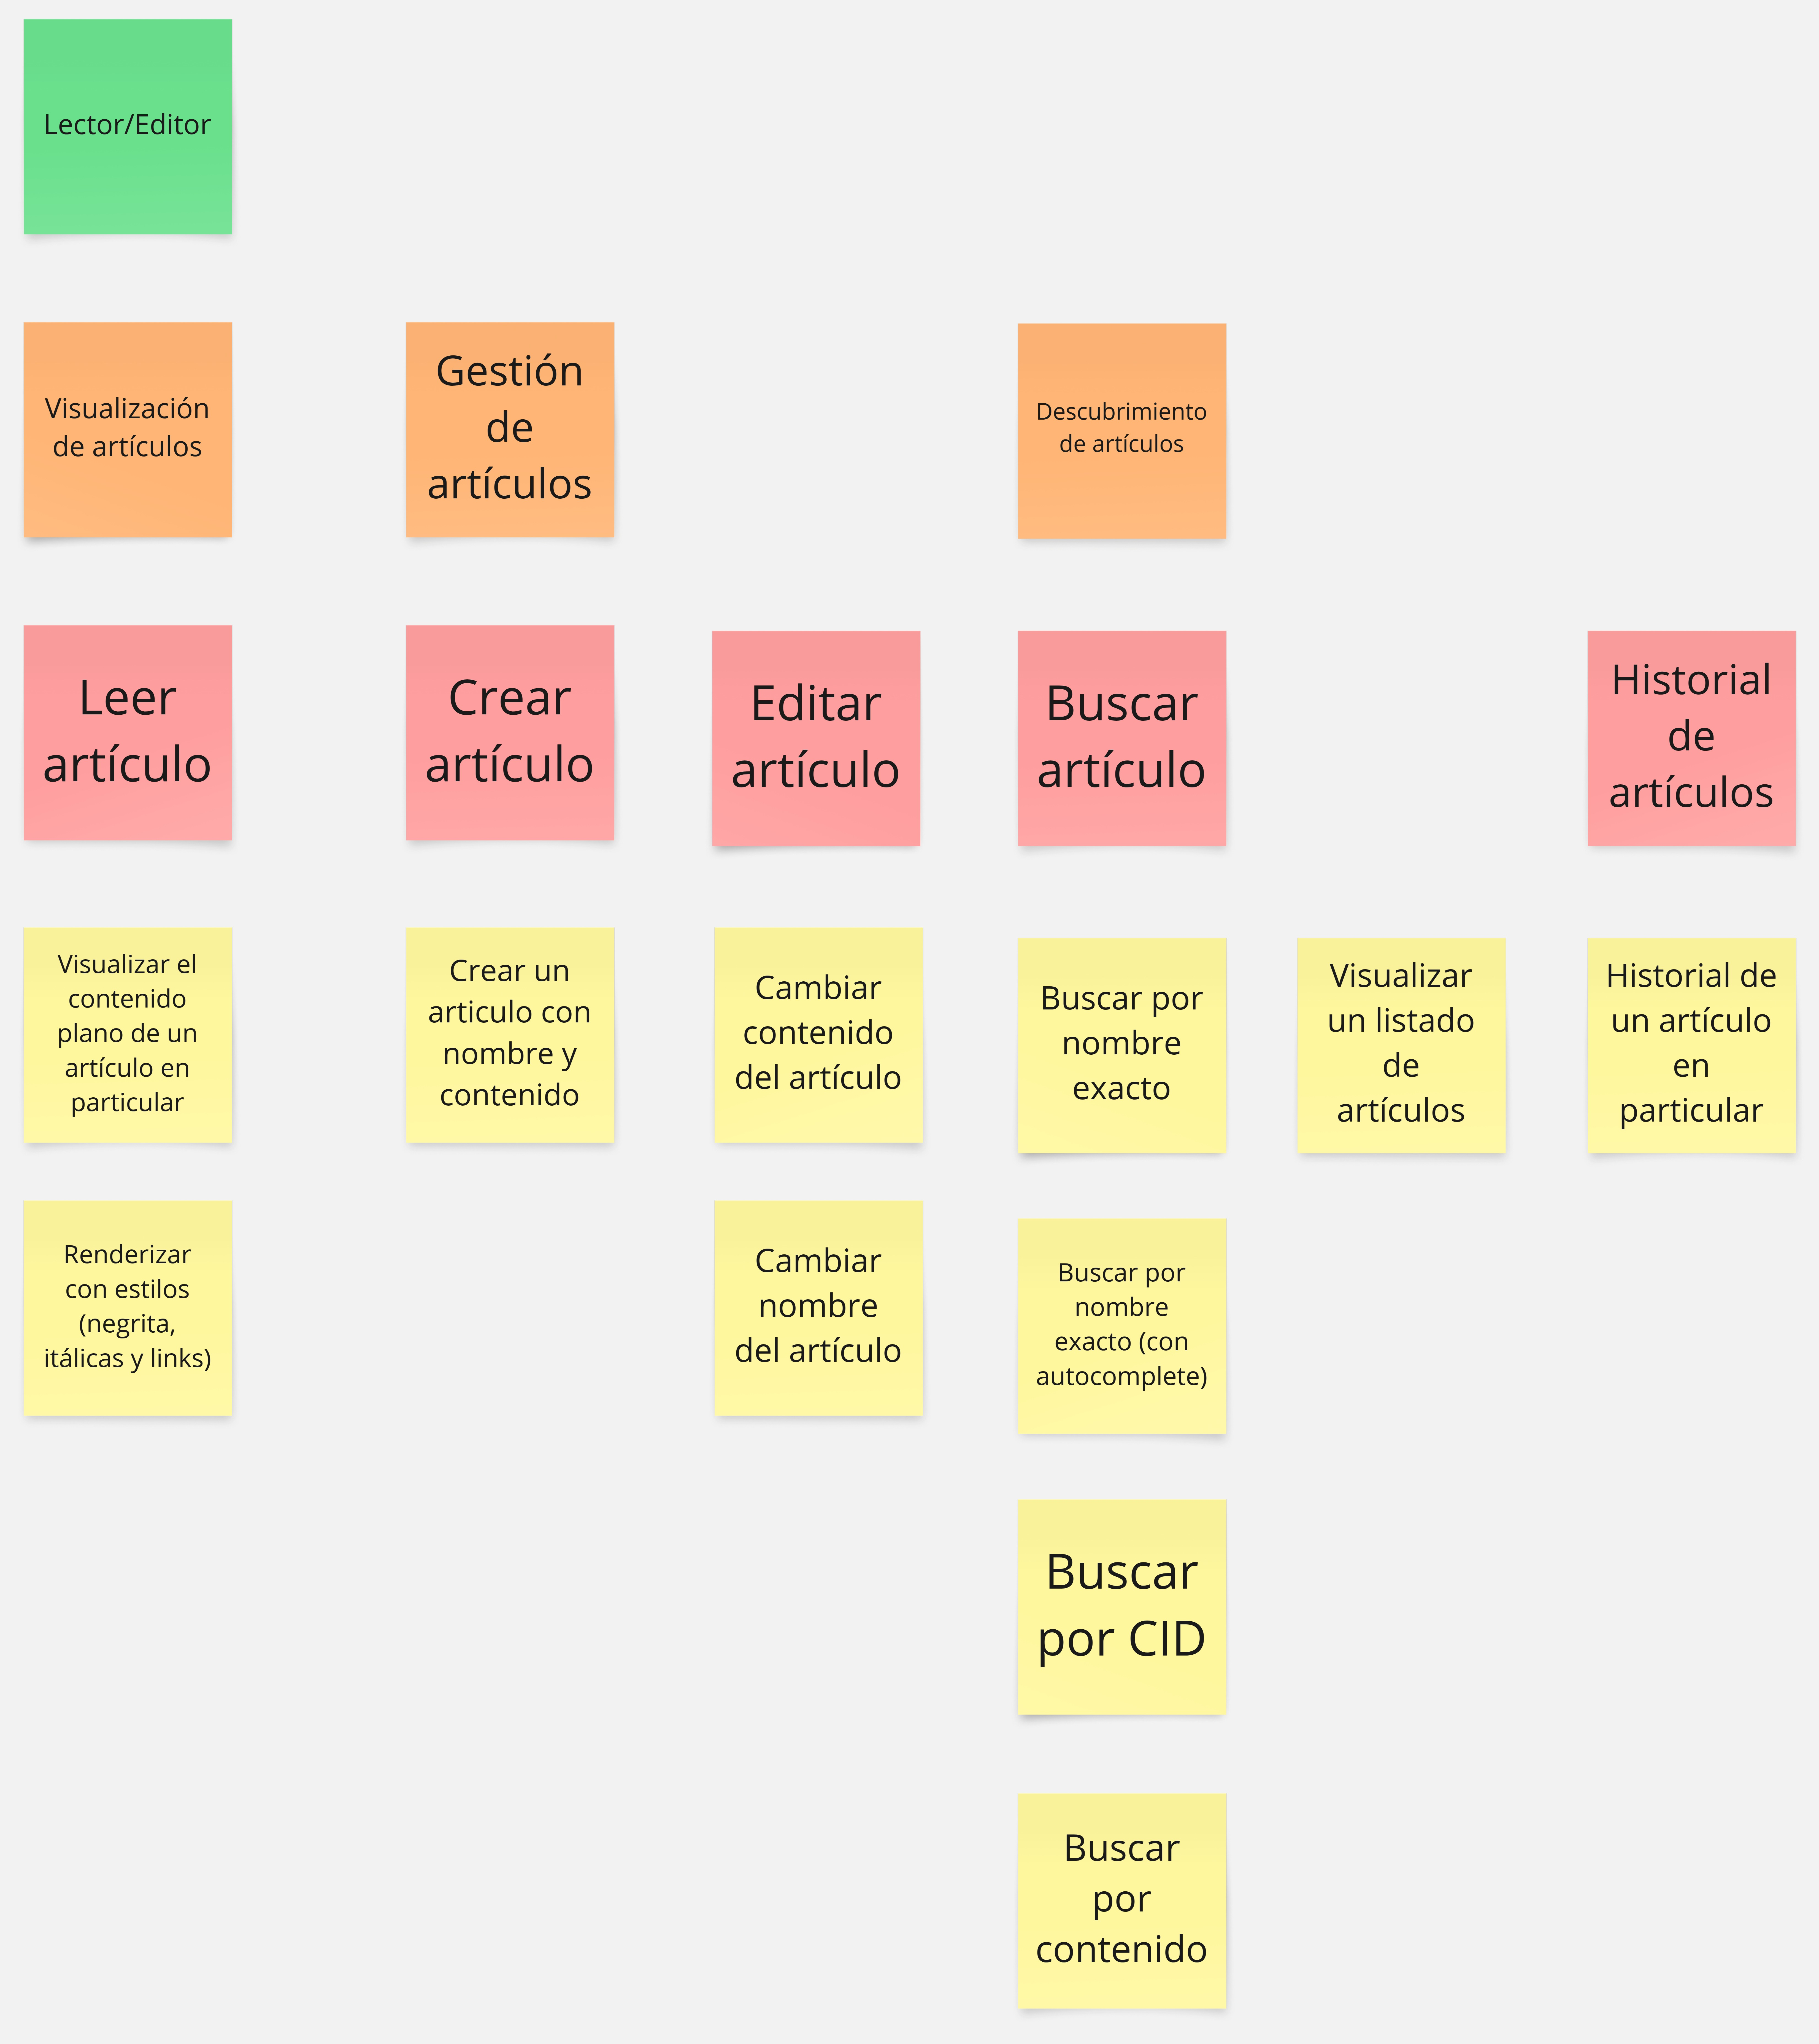
\includegraphics[width=0.5\linewidth]{img/solucion-wiki/usm-wiki.jpg}
    \caption{\textit{User Story Map} del repositorio de conocimiento}
    \label{fig:usm-wiki}
\end{figure}

\paragraph{Arquitectura}

La arquitectura del repositorio de conocimiento fue diseñada de manera independiente del ecosistema utilizado. Se tomó esta decisión para proveer una interfaz común, independiente de su implementación en IPFS y Ethereum. De esta manera, una aplicación puede trabajar sobre una API común e intercambiar implementaciones fácilmente. Esto es útil para la implementación del front-end del repositorio, como se verá más adelante.

En sí, la arquitectura consiste de una o varias \textit{wikis}, dependiendo de la implementación. Cada wiki se identifica con un nombre único que representa un grupo de artículos en conjunto. Cada wiki se representa con una lista de artículos, los cuales son identificados por sus nombres —también únicos. 

Un artículo se compone de un nombre único y no vacío y su contenido. Si bien nuestra implementación utiliza \textit{markdown} \cite{markdown} como formato del contenido, el tipo de contenido es arbitrario e indiferente para la wiki, cualquier tipo de archivo es admisible. Únicamente será tenido en cuenta en el momento en el que la aplicación que interactúe con el contenido lo interprete. En nuestro caso, markdown representa una manera sencilla de enriquecer un texto, lo cual lo hace apropiado para un repositorio de conocimiento comunitario.

\begin{figure}[H]
    \centering
    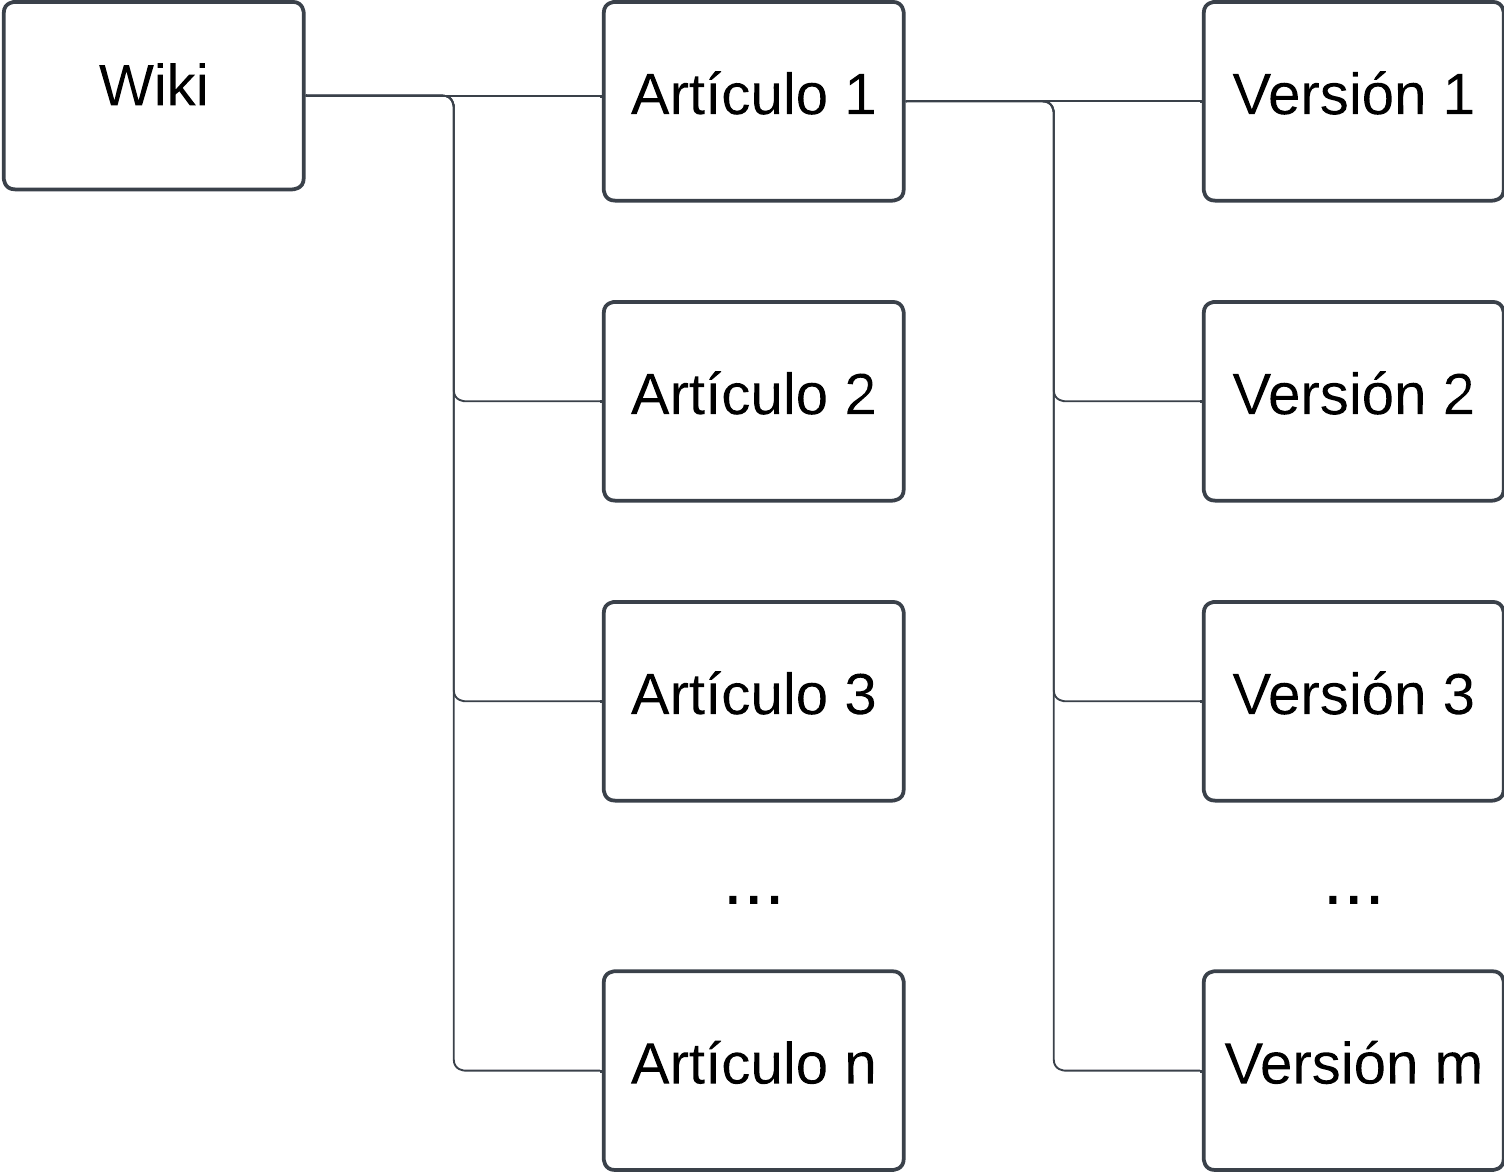
\includegraphics[width=0.5\linewidth]{img/solucion-wiki/arquitectura-wiki.png}
    \caption{Arquitectura general del repositorio de conocimiento.}
    \label{fig:usm-wiki}
\end{figure}

\subparagraph{Representación de un artículo}

Internamente, los artículos pueden editarse en el tiempo, y un usuario debe obtener siempre la última versión. Sin embargo, se debe poder ver versiones anteriores si así lo desea el usuario, por lo que guardar la última versión únicamente no es válido. Es por esto que se decidió representar a un artículo como un nombre, y un conjunto de versiones. Cada versión representa una modificación hecha al artículo. Un artículo nuevo tendrá una única versión, y al hacerle una edición tendrá dos.

Esta iteración de la arquitectura permite a los usuarios ver el historial de versiones, y acceder a cualquiera de ellas. Pero guardar todo un artículo por cada edición puede ser costoso en concepto de almacenamiento. Rara vez un artículo es modificado en su totalidad \cite{wiki-edits-stats}. En cambio, las ediciones que puede sufrir un artículo se deben en su mayoría a la inclusión de contenido nuevo, o la modificación de una sección en particular. Guardar el contenido completo en casos donde los cambios son mínimos resulta ineficiente, y es particularmente negativo en aplicaciones peer-to-peer, donde el contenido se almacena en el lado del usuario.

\subparagraph{Generación de patches}

Como solución para minimizar la información redundante en cada versión, se decidió usar el tipo de algoritmo de \textit{data differencing} \cite{data-differencing}, que consiste en almacenar únicamente los cambios hechos en una versión con respecto a su antecesora, de forma similar a \textit{Git}. Esta lista de cambios forma un \textit{patch}.

Un patch se obtiene al aplicar un algoritmo que reciba el contenido anterior, y el contenido nuevo, y devuelva un patch que pueda ser utilizado posteriormente para reconstruir el contenido. Si bien hay varios algoritmos que logran este objetivo, se decidió utilizar el algoritmo de diff de Myers \cite{myers-diff}, ya que ofrece un punto medio entre compresión, y cómputo necesario para compilar el texto. Este algoritmo es el que utiliza la biblioteca diff-match-patch, creada por Google, que ofrece una interfaz sencilla para lograr generar patches y luego compilar texto en base a ellos.

Calculando los patches de la nueva versión con respecto a la anterior, reducimos el espacio necesario para almacenar un artículo con todas sus versiones.  Hay casos en los que un patch puede tener un tamaño mayor al de simplemente almacenar una copia del nuevo contenido. Sin embargo, estos casos no son frecuentes en usos comunes y decidimos despreciarlos, aunque puede ser una posible mejora para optimizar más aún el espacio utilizado.

Por otra parte, ya que cada versión no tiene toda la información, se necesitan todas las versiones anteriores para compilar el contenido resultante. Esto puede ser una desventaja en archivos con muchas ediciones, ya que requieren de mayor cómputo para compilar, específicamente \texttt{O(n)}, donde \texttt{n} es la cantidad de versiones que tiene el artículo. Para mejorar esto, una posible mejora consiste en fijar un número máximo de patches consecutivos que, al superarse, indica que la siguiente versión debe contener el contenido completo. De esta manera se acota la cantidad de iteraciones que puede tomar la compilación de un artículo.

La nueva iteración de la arquitectura apunta a tener una lista de versiones, que a su vez contengan el patch con las diferencias con la versión anterior. Pero como se verá en la siguiente sección, esta solución no es lo suficientemente resiliente.

\subparagraph{Concurrencia}

En las redes peer-to-peer es común que la replicación de contenido lleve un tiempo no despreciable. Esto puede generar problemas, ya que dos nodos pueden publicar contenido que entre en conflicto, de la misma manera que dos cambios pueden generar un \textit{merge conflict} en Git. En el mejor de los casos, ambos nodos publican
contenido que no entra en conflicto entre sí, y por lo tanto la compilación se puede realizar sin problemas. En el caso contrario, puede dejar el artículo en un estado inválido, imposible de compilar y por lo tanto, inaccesible.

Yendo a nuestro caso de uso, el problema planteado previamente puede entrar en conflicto de dos maneras:
\begin{enumerate}
    \item Al crear un articulo
    \item Al editar un artículo
\end{enumerate}

Por lo tanto, es necesario una solución que mitigue estos problemas.

Para el caso de la creación de dos artículos con en mismo nombre, se delega en cada ecosistema la responsabilidad de detectar estos casos y actuar en consecuencia. La implementación de cada ecosistema contiene más información para tomar una decisión optimizada al respecto, la cuál se verá en secciones posteriores. En cambio, el problema de la edición de un artículo de forma concurrente puede ser resuelto a nivel arquitectura.

\subparagraph{Árbol de versiones}

Hasta ahora, cada versión se agrega a una lista de versiones, y se asume que cada versión se basa en la anterior. Cuando ocurre un conflicto de concurrencia entre versiones, esto no aplica por las razones dadas previamente. Por lo tanto, es necesario que cada versión tenga un ID para que las versiones posteriores puedan mantener registro de su versión padre, es decir, la versión sobre la que se basa. Todas las versiones tienen padre, excepto la versión inicial. Cuando dos versiones se crean en base a una misma versión padre, se genera una bifurcación. Por lo tanto, las versiones pasan a formar un árbol.

En arquitecturas tradicionales, la generación de IDs suele hacerse por la misma base de datos, de manera incremental. Esto no genera problemas ya que el servidor decide en que orden tomar las versiones. En una aplicación distribuida, esto no es conveniente, ya que dos nodos pueden generar el mismo ID por la misma razón por la que pueden generar versiones conflictivas. La solución elegida fue usar \texttt{UUID}s \cite{uuid}, que se generan sin necesidad de centralizar la decisión, y tienen una probabilidad de colisión casi nula.

Una problemática que trae tener distintas ramas de versiones es que la compilación del contenido deja de ser trivial, ya que hay múltiples posibles últimas versiones, dependiendo de la rama que se elija. Para resolver esto es necesario definir una heurística que elija la rama principal del artículo de forma determinista.

\begin{figure}[H]
    \centering
    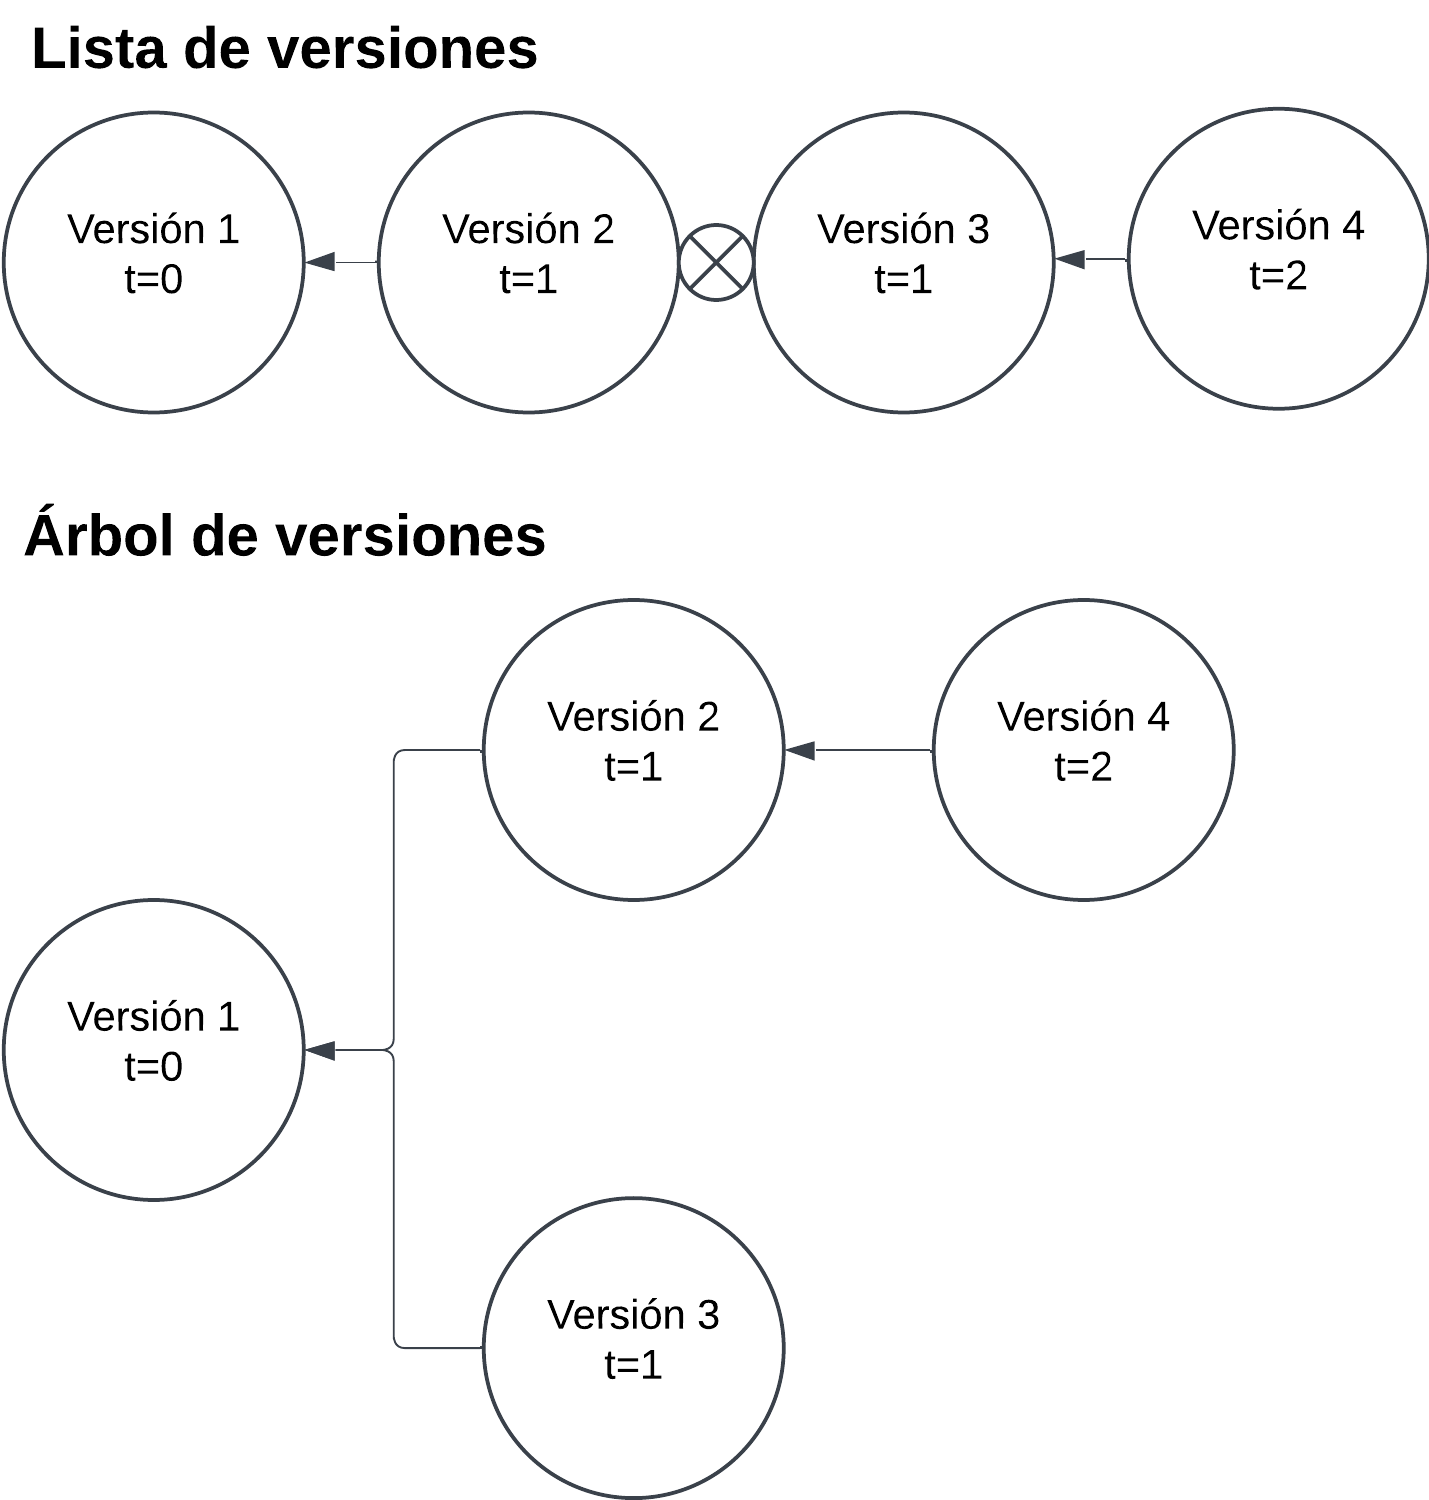
\includegraphics[width=0.5\linewidth]{img/solucion-wiki/arbol-versiones.png}
    \caption{Ambas maneras de almacenar versiones. En este caso, \texttt{t} es un momento en el tiempo en el que todas las bases de datos están sincronizadas. En el primer caso, cuando \texttt{t=1} en ambas versiones, significa que hay un conflicto ya que ambas se basan en la misma versión padre. En el árbol, ese problema se mitiga.}
    \label{fig:usm-wiki}
\end{figure}

\subparagraph{Elección de rama principal}

Una de las decisiones tomadas respecto al árbol de versiones, es que los usuarios sólo puedan modificar la última versión “principal”, es decir; un usuario no podrá editar en base a una versión arbitraria. Teniendo en cuenta esto, es fácil deducir que las ramas no principales o secundarias tendrán a lo sumo una versión en la mayoría de los casos. Esto es debido a que los demás usuarios que no hayan causado la colisión elegirán una rama principal, por lo tanto las demás ramas dejarán de recibir versiones nuevas. Elegir la rama de mayor cantidad de versiones será parte de la heurística para elegir la rama principal.

Sin embargo, esta decisión no es exhaustiva, ya que puede haber dos ramas con la misma longitud. De hecho, este caso es muy común debido a que dos usuarios que crean una nueva versión en base a la misma versión padre generan dos ramas del mismo tamaño. Para tomar una decisión que sea determinista e igual en todos los nodos, se decidió tomar la antigüedad de la última versión de cada rama como parámetro para la heurística. La rama mas antigua será considerada la rama principal. La antigüedad de una rama es decidida por una marca de tiempo o \textit{timestamp} grabada en el mismo nodo que crea la rama, y es enviado como parte de la versión a los demás nodos. Esto trae una desventaja en cuánto a seguridad, ya que un nodo puede falsificar un timestamp y así tener prioridad siempre, pero es mejorable utilizando algoritmos para crear timestamps en un sistema distribuido \cite{distributed-timestamps}.

\begin{figure}[H]
    \centering
    \begin{minipage}{0.9\linewidth}
        \lstset{
            basicstyle=\ttfamily\small,
            frame=single,
            captionpos=b
        }
        \begin{lstlisting}
type VersionID = string;

type Version = {
  id: VersionID;
  date: string;
  patch: Patch;
  parent: VersionID | null;
};\end{lstlisting}
    \end{minipage}
    \caption{Propiedades de una \texttt{Version}}
    \label{fig:version-type}
\end{figure}

Una vez elegida la versión principal, se considera como rama principal a todas las versiones que entren en la cadena de padres, empezando por la versión principal hasta llegar a la versión raíz. De esta forma, sabemos que la rama principal siempre se podrá compilar, generando una red mucho más resiliente a cambios concurrentes. 
Por último, las versiones que no sean parte de la rama principal también podrán visualizarse. Se tomó esta decisión para permitir que los usuarios que hayan subido una versión por fuera de la rama principal puedan ver el contenido que editaron y, en todo caso, editar la nueva versión principal con el mismo.

\subsubsection{Mensajero en tiempo real}

Este caso se enfoca en la capacidad de la infraestructura de enfrentarse a situaciones de \textit{tiempo real} como puede ser un chat de texto o de audio. En particular, nos centramos en el caso de chats de texto para un grupo de usuarios en donde los mensajes sean públicos.

\paragraph{Requisitos funcionales}

\begin{itemize}
    \item \textbf{Usuarios:} se deben contar con usuarios que puedan iniciar sesión con una clave.
    \item \textbf{Grupos públicos:} grupos de chat de texto, donde cualquier usuario puede ingresar y ver los mensajes del resto, así como también participar enviando sus propios mensajes.
    \item \textbf{Respuestas:} un usuario debe poder responder mensajes anteriores dentro de un mismo chat.
\end{itemize}

\begin{figure}[H]
    \centering
    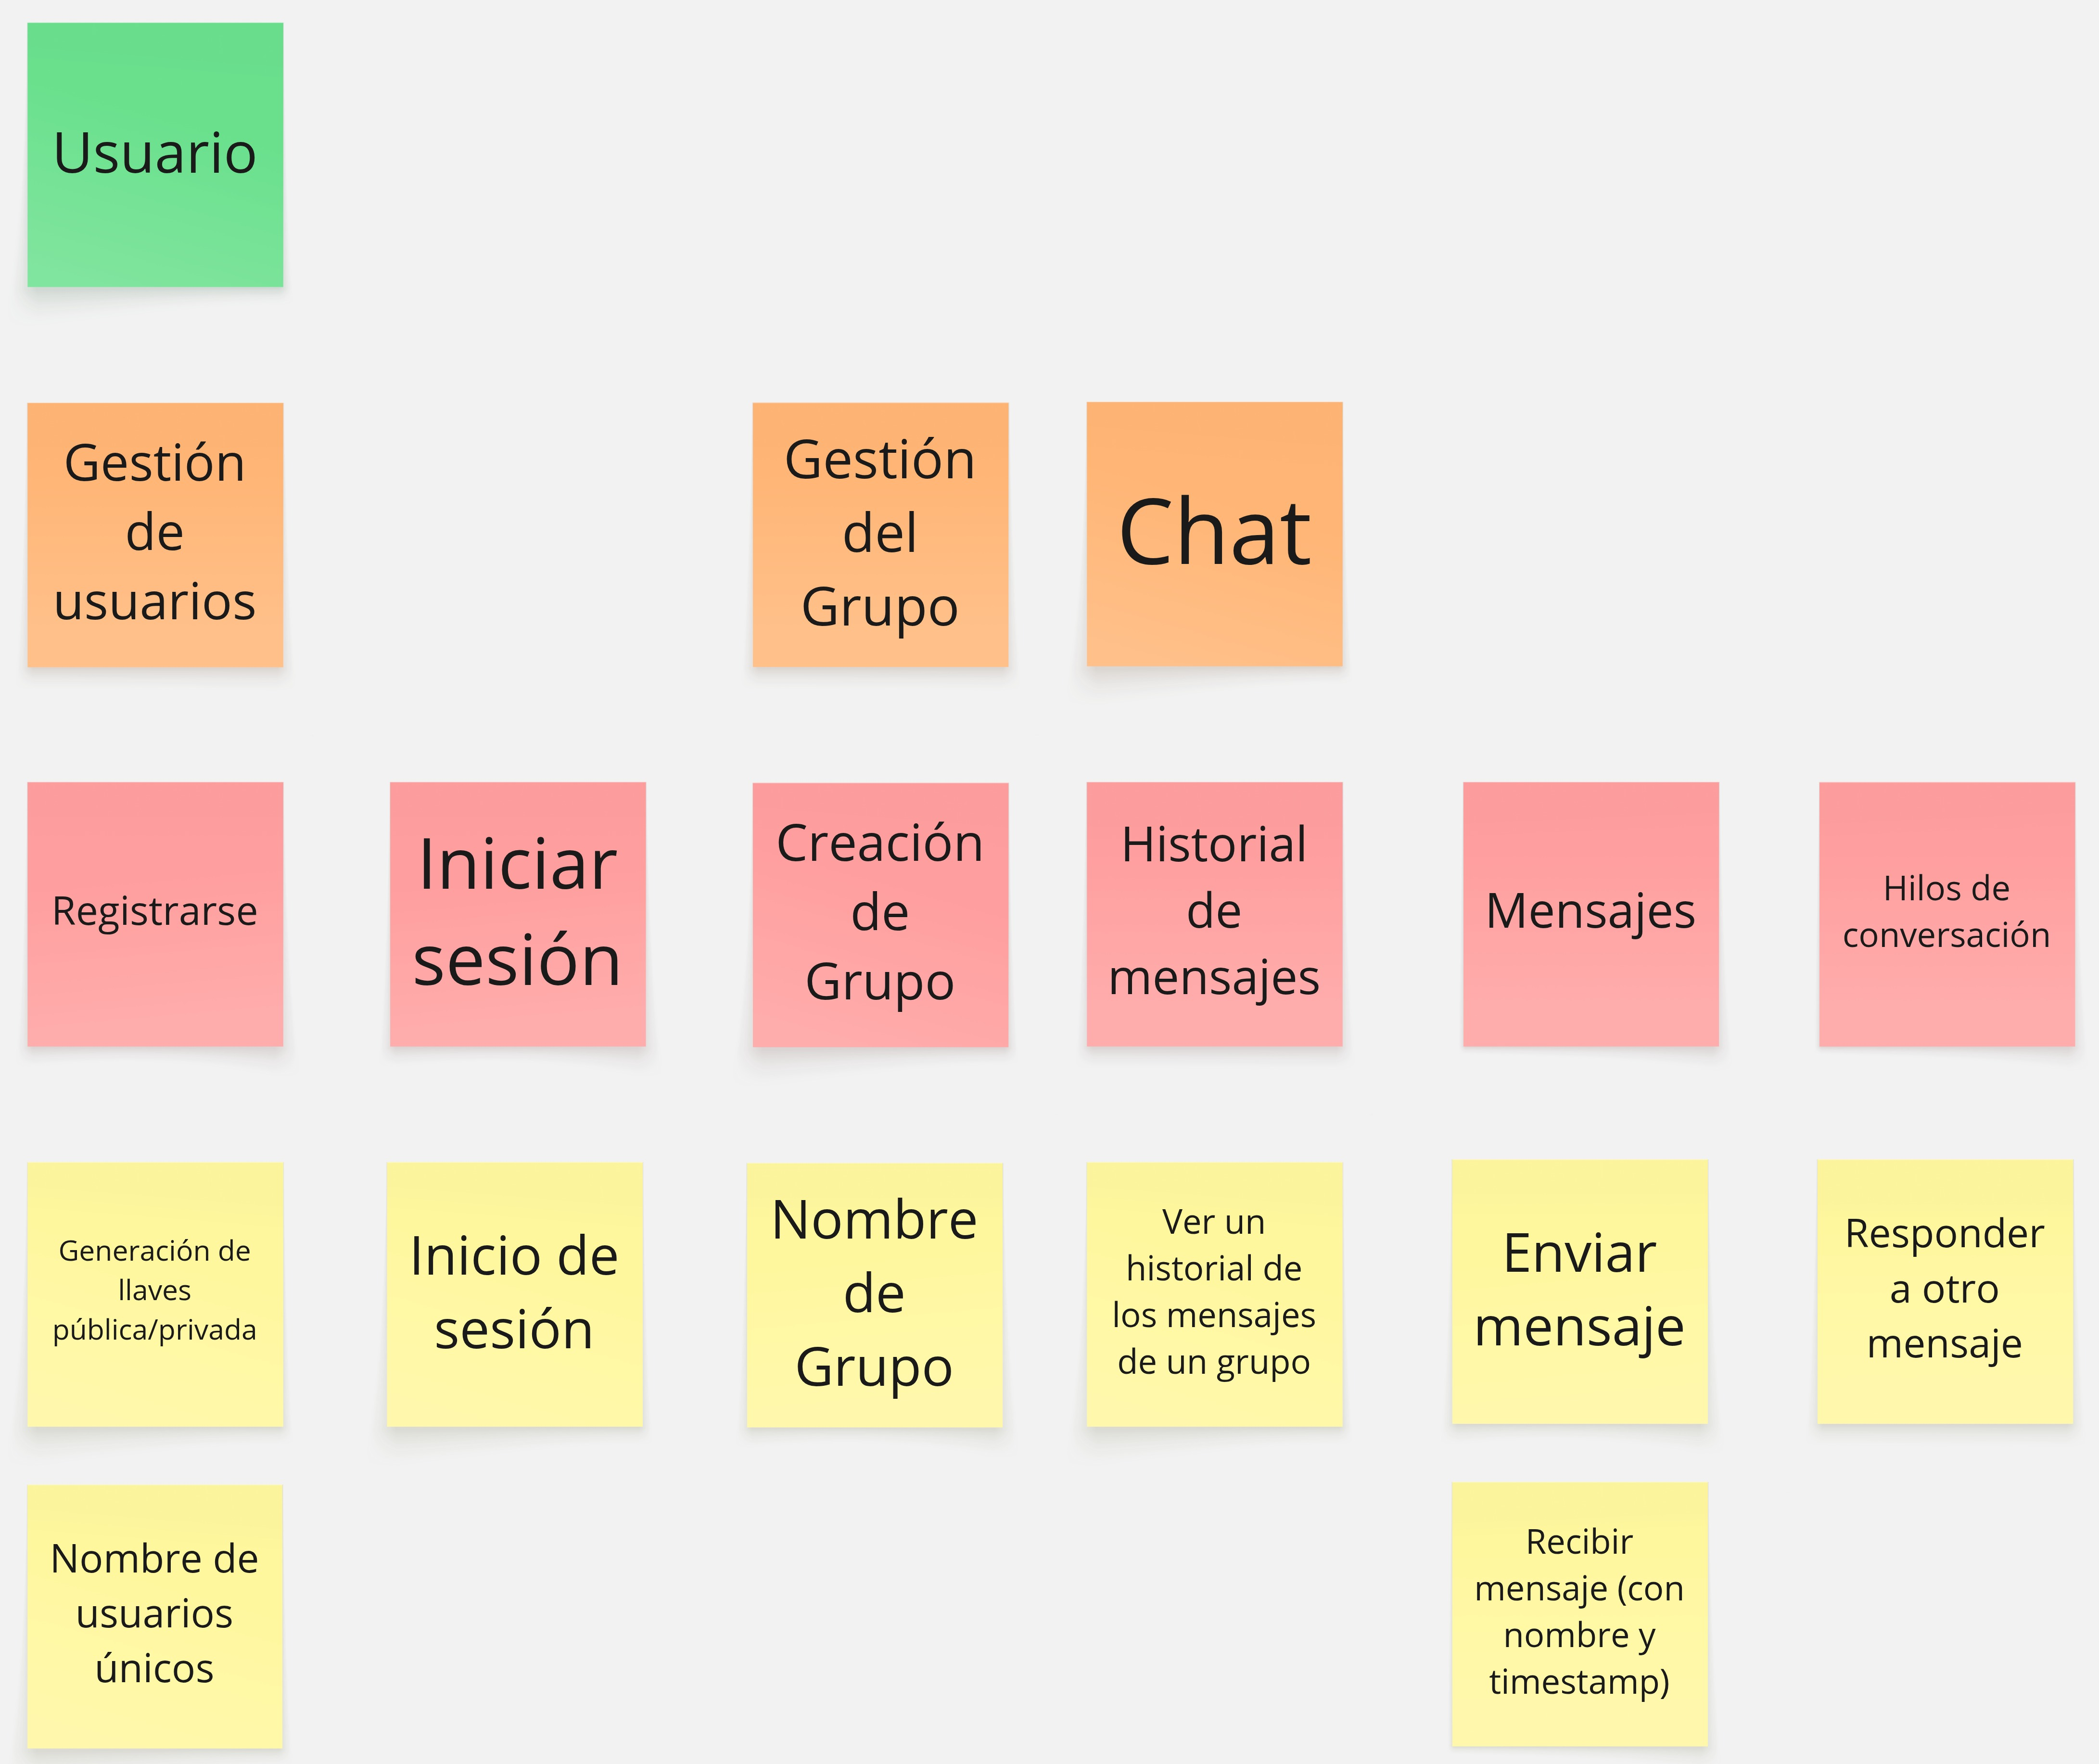
\includegraphics[width=0.5\linewidth]{img/usm-mensajero.jpg}
    \caption{\textit{User Story Map} del mensajero en tiempo real}
    \label{fig:enter-label}
\end{figure}

\paragraph{Arquitectura}

La arquitectura para un mensajero es mucho más sencilla que la del repositorio de conocimiento. Consta de un grupo de chats, que a su vez contienen todos los mensajes. Cada mensaje contiene el texto enviado, el usuario que lo envió, un \textit{timestamp} del momento de su envío, entre otras cosas.

\subparagraph{Aliases} En las implementaciones que se verán posteriormente, se determina que la manera de identificar a un usuario será mediante un ID similar a un hash en ambos casos. Esto es común para sistemas descentralizados, pero vuelve difícil diferenciar los usuarios en un chat. Para solucionar esto, se decidió agregar un alias que identifique al usuario, que no tenga que ser único y pueda ser cambiado. Su implementación varía dependiendo del ecosistema, pero en ambos es parte del objeto \texttt{ChatMessage} que almacena cada chat.

\subparagraph{Respuestas} Se decidió identificar cada mensaje mediante un identificador, de manera tal que se pueda indicar el "padre" de un mensaje, o sea, el mensaje al que se le está respondiendo.

\begin{figure}[H]
    \centering
    \begin{minipage}{0.9\linewidth}
        \lstset{
            basicstyle=\ttfamily\small,
            frame=single,
            captionpos=b
        }
        \begin{lstlisting}
export type ChatMessage = {
  id: string;
  parentId: string;
  sender: string;
  senderAlias: string;
  message: string;
  timestamp: number;
};\end{lstlisting}
    \end{minipage}
    \caption{Propiedades de un \texttt{ChatMessage}}
    \label{fig:version-type}
\end{figure}

\subsection{Proceso de descubrimiento}

Durante la implementación de los casos de uso para cada ecosistema, se fue desarrollando un mejor entendimiento de lo que se estaba creando. Logrando así generar distintas abstracciones que representan la infraestructura general para la implementación de los casos de uso.

Para cada ecosistema hay 2 principales infraestructuras en acción. La infraestructura de despliegue y la infraestructura de aplicación.

La \textbf{infraestructura de despliegue} es la encargada del \textit{hosting} de una aplicación web. Con esta se distribuye y permite el acceso a lo que es el \textit{front-end} de las aplicaciones, como también el código para el funcionamiento de la aplicación, si se trata de una aplicación no estática. Cualquier aplicación que desee ser accedida por la web va a hacer uso de esta infraestructura, como es el caso del sitio web informativo.

La \textbf{infraestructura de aplicación} es la encargada de la lógica de la aplicación, como es el almacenamiento de datos, como la conexión entre pares. Aplicaciones que requieran de mantener un estado y permitir la modificación de parte de los usuarios van a necesitar hacer uso de esta infraestructura, como es el caso del repositorio de conocimiento y mensajero en tiempo real.

% TODO: (Mover a IPFS esto, ya que no se hicieron abstracciones en blockchain)
Al lograr encontrar estas abstracciones, se permite que generar nuevos casos de uso sea mucho más fácil, ya que la mayoría de la lógica sobre el el ecosistema se encuentra encapsulada dentro de ellas, logrando que el desarrollo de un nuevo caso de uso se concentre únicamente en sus requisitos y no en el ecosistema en el que se encuentra.

A continuación se va a explicar como se componen y funcionan ambas infraestructuras en cada ecosistema.

% TODO: (Explicar que lo que hicimos son packages)

\subsection{IPFS}

\subsubsection{Infraestructura de despliegue}

En IPFS, es posible desplegar una aplicación web subiendo un directorio con todos los archivos estáticos necesarios para el funcionamiento en un navegador, incluyendo el código necesario a nivel aplicación. Esto se puede realizar manualmente mediante cualquier cliente de IPFS, como Kubo\cite{kubo} o Helia\cite{helia}, y devuelve un \textit{content identifier} (CID) \cite{cid} que representa esa versión de la aplicación.

Cualquier usuario puede publicar su sitio web en la red de IPFS a través de un nodo local de manera gratuita y poco tiempo. IPFS provee un tutorial en su página de cómo realizarlo \cite{ipfs-static-website}. A continuación se detallará las implicaciones que tiene desplegar una aplicación web de esta manera, y que alternativas existen para publicar en IPFS.

Al subir un archivo —por ejemplo, código HTML— su contenido se inserta en una función de hash, y así se obtiene su CID. Desde ese momento, cualquier nodo que desee obtener el archivo puede encontrarlo utilizando dicho CID. Sin embargo, no se asegura la persistencia del archivo, y dejará de ser accesible luego de un tiempo. Esto se debe al \textit{garbage collector} \cite{garbage-collector} implementado por IPFS, que desecha datos para liberar almacenamiento de forma arbitraria. Por esta razón existe el concepto de \cite{pinning}: \textit{"pinear"} un archivo o directorio significa instruir al nodo IPFS para que trate dicha información como esencial y, por lo tanto, no lo descarte. 

No obstante, pinear un archivo o directorio no asegura su disponibilidad indefinida en el tiempo, ya a que esta depende de que el nodo que lo tiene pineado esté activo, o de que otros nodos que hayan accedido al archivo y aún lo tengan en su caché. Para mejorar la disponibilidad de un archivo, lo ideal es que varios nodos pineen el contenido, de modo que otro nodo que desee obtener el contenido pueda hacerlo desde cualquiera de ellos.

Para lograr que el contenido persista en la red sin necesidad de que el nodo local esté activo, existen opciones para delegar el pineo del archivo o directorio. Existen servicios de pinning y clusters colaborativos, que actúan pineando los archivos en múltiples nodos, aumentando no solo su disponibilidad sino también su distribución, y por ende logrando un acceso más rápido al contenido.

\paragraph{Servicios de \textit{pinning}}

La manera más fácil de asegurarse que los datos estén disponibles y se persistan es usar un servicio de \textit{pinning} \cite{pinning-services}. Estos servicios cuentan con varios nodos que pinnean archivos. De esta manera, ya no es necesario contar con un nodo local que los aloje. Algunos ejemplos de servicios de pinning incluyen Fleek \cite{fleek} y Pinata \cite{pinata}.

Desde el punto de vista de las aplicaciones estrictamente comunitarias, estos servicios no van de la mano con su filosofía. Por un lado, los servicios de \textit{pinning} tienen un modelo gratis con funcionalidad limitada o capacidad de almacenamiento limitado. Por otro lado, se depende de estos servicios, lo que en esencia centraliza el proceso de despliegue de la aplicación o sitio web. Si por algún motivo el servicio dejara de pinear los archivos, estos pueden dejar de estar disponibles en la red IPFS, e incluso pueden perderse por completo. Esto rompe completamente con la naturaleza de aplicaciones descentralizadas y pasa a tener una centralización tercerizada similar a utilizar un \textit{cloud hosting}.

\paragraph{Clusters colaborativos}

Un \textit{cluster} es un grupo de nodos de IPFS que actúan en conjunto para pinear un contenido. Funcionan sincronizando su \textit{pin set}, o sea, su lista de archivos y directorios pineados en un momento dado. Un cluster \textit{colaborativo} sigue esta premisa, pero permite que los usuarios puedan colaborar con su nodo local para el pineo de la aplicación sin tener la posibilidad de modificar los archivos, la cuál es delegada a nodos especiales que tienen la capacidad de orquestar el cluster en conjunto. Así, se logra que la misma comunidad mantenga en servicio el mecanismo de despliegue de la aplicación, lo cuál es acorde a la filosofía de aplicaciones comunitarias.

Actualmente, esta alternativa es poco explorada, por lo tanto no existe una forma fácil de creación, seguimiento y descubrimiento de estos clusters. IPFS cuenta con una página con clusters conocidos con los cuales se puede colaborar \cite{collaborative-clusters}, pero la cantidad es limitada.

Por otro lado, el principal problema es que los clusters obligan a los nodos a "pinear" la totalidad de sus archivos, lo cuál puede significar un uso excesivo de almacenamiento necesario para colaborar. Hacer sharding sobre el pin set, o sea, pinear parte del contenido de un cluster, es posible utilizando los parámetros de replicator\_min\_max al agregar un pin, que fijan un límite mínimo y máximo sobre la cantidad de nodos que tienen ese pin. Sin embargo, no es recomendado para clusters colaborativos debido a la falta de \textit{proof of storage} \cite{cluster-sharding} \cite{collaborative-clusters-setup}. Esto se debe a que, debido a la manera en la que fue diseñada la arquitectura de IPFS, un nodo no confiable puede falsificar la lista de archivos que está pineando, por lo que hay una posibilidad de que una parte del contenido no esté en ninguno de los nodos, y por ende el contenido esté incompleto.

\paragraph{Acceso y mutabilidad}

Para buscar un contenido, un nodo de IPFS realiza una búsqueda a través de su CID, el cual es único. Debido a que es único, el CID cambiará si el contenido del sitio web o aplicación web cambia, ya que el contenido será distinto. Esto vuelve el proceso de despliegue altamente impráctico, ya que se necesitaría compartir un nuevo CID cada vez que se actualice una página.

Este problema puede ser resuelto con la ayuda de \textit{punteros mutables}. Estos punteros son un objeto de IPFS que apunta a un CID determinado, previamente elegido por el usuario. El CID al que apunta el puntero puede ser cambiado, por lo tanto permiten compartir la dirección del puntero una única vez y actualizar el CID al cuál apunta cada vez que se haga un cambio.

\subparagraph{IPNS}

InterPlanetary Name System (IPNS) \cite{ipns} es un sistema que permite crear  punteros mutables y obtener su dirección en forma de CIDs conocidos como \textit{names} o \textit{nombres de IPNS}. Estos nombres de IPNS pueden considerarse como enlaces que pueden actualizarse, conservando al mismo tiempo la verificabilidad del content addressing.

Un nombre de IPNS es un hash de una \cite{ipns-hash} clave pública. Está asociado a un \textit{IPNS record} \cite{ipns-record} que contiene la ruta a la que se vincula, entre otra información. El titular de la clave privada puede firmar y publicar nuevos registros en cualquier momento.

Es posible utilizar IPNS con uno de estos posibles enfoques:
\begin{itemize}
    \item \textbf{Consistencia:} garantizar que los usuarios siempre resuelvan el último registro de IPNS publicado, a riesgo de no poder resolverlo.
    \item \textbf{Disponibilidad:} resolver un registro de IPNS válido, a costa de potencialmente resolver un registro desactualizado -o sea, con un CID previo.
\end{itemize}

El registro IPNS se encuentra a través de la \textbf{Distributed Hash Table} (DHT) \cite{dht}. Todos los nodos de IPFS participan alojando colaborativamente el contenido de la DHT. Por lo tanto, el DHT actúa como un "directorio" descentralizado, donde la clave pública es un identificador. Esta tabla ayuda a localizar el registro IPNS que apunta al contenido deseado, entre otras funciones. Para entender mejor cómo IPNS funciona se puede consultar la documentación de IPFS.

IPNS es una buena forma de obtener mutabilidad dentro de IPFS. Una vez que se aloja un contenido en IPFS y se apunta a él mediante un \textit{nombre} de IPNS, el mayor problema pasa a ser la manera de acceder a IPNS en sí. El hecho de que los names sean hashes alfanuméricos, y no nombres legibles o memorables para humanos, representa una dificultad adicional a la hora de alojar un sitio web al cuál los usuarios puedan acceder fácilmente. A continuación se analizará dos alternativas para solucionar este problema.

\begin{figure}[h]
\centering
\fbox{\texttt{/ipns/k51qzi5uqu5dhkdbjdsauuyk5iyq82uzpjb0is3x6oy9dcmmr8dbcezv7v9fya}}
\caption{Ejemplo de la dirección de un nombre de IPNS}
\end{figure}

\subparagraph{DNSLink}

IPNS no es la única forma de crear mutable pointers en IPFS. DNSLink \cite{dnslink} utiliza registros \textit{DNS TXT} para asignar un nombre DNS (por ejemplo, un dominio) a una dirección IPFS o a un \textit{IPNS name}. Como uno puede editar sus registros DNS, puede usarlos para que siempre apunten a la última versión de un objeto en IPFS.

DNSLink actualmente es mucho más rápido que IPNS, utiliza nombres legibles por humanos y también puede apuntar a nombres de IPNS. A pesar de ello, tiene un problema muy fundamental y es que se utiliza el protocolo \textbf{DNS}, el cual tiene claras deficiencias con la filosofía de aplicaciones comunitarias.

La más importante es que, aunque DNS tenga claras ventajas, como ser un sistema distribuido y escalable, es también un sistema algo centralizado. Las autoridades centrales como \textit{ICANN} gestionan las raíces del DNS. Esto hace que un registro DNS sea fácil de censurar, a nivel de registrador como también a nivel \textit{ISPs}.

\subparagraph{ENS}

\textbf{Ethereum Name Service (ENS)} \cite{ens}, es el protocolo de nombres descentralizado que se basa en blockchain \textit{Ethereum}. Funciona de manera similar a DNS, en el sentido de que los nombres ENS resuelven a nombres legibles para humanos. Como esto se computa en la blockchain de Ethereum, es seguro, descentralizado y transparente. Está diseñado específicamente para traducir identificadores como direcciones de billeteras de criptomonedas, hashes, metadata, entre otros, incluyendo direcciones de IPFS.

Es posible configurar un registro ENS para que se resuelva automáticamente la dirección IPNS, proporcionando nombres legibles para humanos que son más fáciles de compartir y acceder, y solucionando el principal problema de IPNS hasta este punto. Además, cuando se quiera actualizar el contenido, no será necesario modificar el registro ENS en sí, ya que siempre se va a apuntar al mismo nombre de IPNS.

Cabe aclarar que adquirir un dominio ENS tiene un costo, que depende de varios factores \cite{ens-price}:
\begin{itemize}
    \item El largo del nombre. Un nombre con menos caracteres tiende a tener un valor mayor.
    \item Cuán reciente expiró la licencia del dominio. Si un dominio expiró recientemente, se le aplica un precio \textit{premium} que decrece con el tiempo. Un dominio con mayor uso aumenta su precio.
    \item El valor del gas actual, que depende de la congestión de la blockchain.
\end{itemize}

\subparagraph{Acceso desde un navegador}

Por último, se necesita una manera de acceder a los archivos alojados en IPFS. En navegadores que soportan IPFS y ENS —como Opera \cite{opera-ipfs} y previamente Brave \cite{brave-ipfs}— se puede acceder directamente. En la mayoría de los navegadores, sin embargo, esta no es una opción. Para lograr un mayor alcance que incluya estos navegadores, se requiere el uso de una \textit{IPFS gateway} \cite{ipfs-gateway}.

Una IPFS gateway es un nodo que recibe requests HTTP que contienen una dirección de IPFS, busca el contenido en la red de IPFS, y lo devuelve en una HTTP response. Esto es útil tanto para archivos como para directorios. Algunas gateways tienen la funcionalidad de mostrar una página web de manera correcta cuando un directorio tiene la estructura indicada. Esto nos es particularmente útil para poder mostrar una página moderna de la misma manera que se haría utilizando un servidor HTTP.

Una lista de gateways disponibles puede obtenerse utilizando el Public Gateway Checker \cite{public-gateway-checker} proporcionado por IPFS.

\begin{figure}[h!]
    \centering
    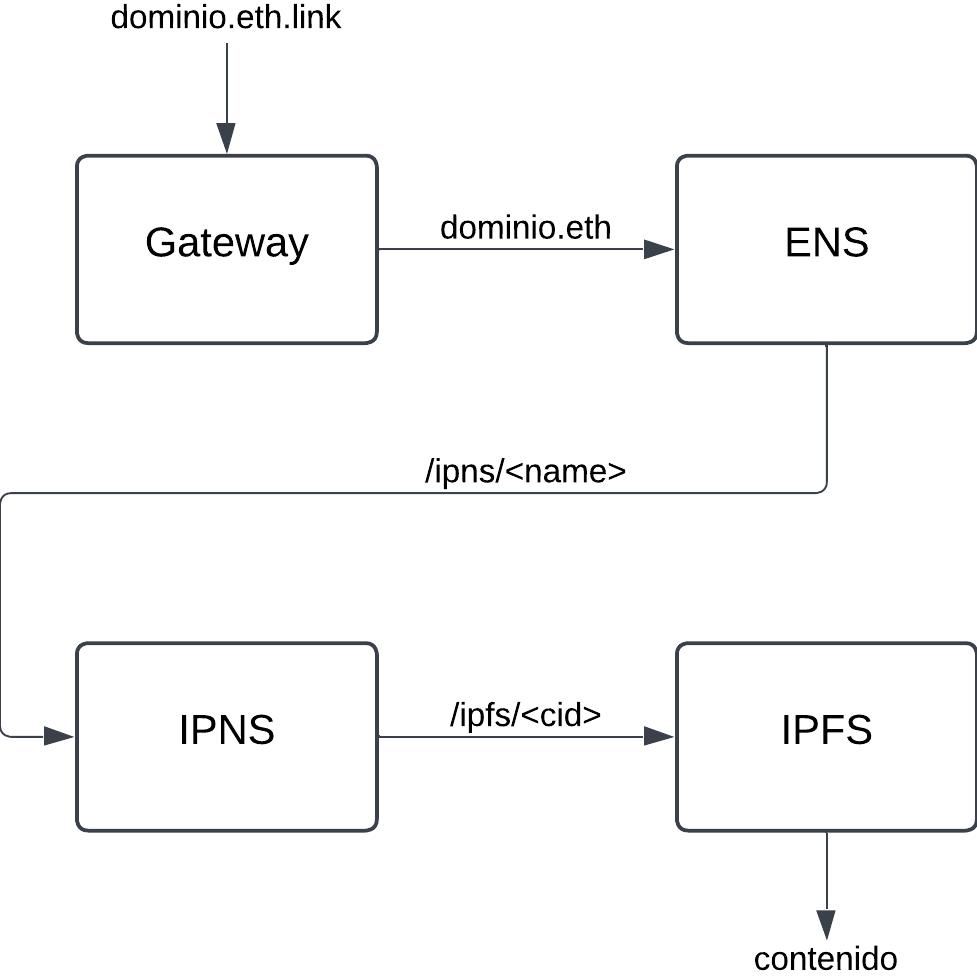
\includegraphics[width=0.5\linewidth]{img/solucion-ipfs/traduccion-dominio.png}
    \caption{Mapa de la traducción de un dominio al contenido de IPFS}
    \label{fig:traduccion-ipfs}
\end{figure}

\paragraph{Despliegue continuo}

En un proyecto de aplicación web centralizada, es común automatizar el proceso de despliegue con cada cambio que se realiza. Normalmente este proceso se activa con cada nuevo commit en una rama de Git especifica, e incluye todas las etapas necesarias para convertir el contenido de un repositorio Git en código estático listo para ser desplegado. También puede incluir más pasos que incluyan actualizaciones en el backend.

Yendo al caso específico de aplicaciones web comunitarias, el script debe ser ejecutado en los nodos confiables, ya que una \textit{Github action} no puede utilizar un nodo IPFS que requiera puertos abiertos. En este tipo de aplicaciones, al tener una jerarquía mayormente horizontal, no hay un servidor central que orqueste esta actualización, sino que se necesita que cualquier nodo confiable pueda actualizar su contenido e instruir a los nodos colaborativos para actualizar su contenido de igual forma. Todo esto debe ser posible incluso cuando los nodos no reciben la actualización al mismo tiempo, es decir, no debe haber \textit{race conditions}.

Una forma de lograr esto es, por ejemplo, utilizar un algoritmo de elección de líder u otro algoritmo distribuido para elegir el nodo responsable de indicar el nuevo contenido a pinear al resto de nodos en el cluster. Sin embargo, esta manera de realizar la actualización implica una capa adicional de complejidad que no es necesaria debido a la naturaleza de IPFS.

Como ya se ha mencionado, si dos nodos suben el mismo contenido, obtendrán el mismo CID. Esto puede ser utilizado para que cualquier nodo confiable pueda actualizar el contenido y el nombre de IPNS independientemente del resto de los nodos confiables. Cuando se detecte un cambio nuevo, el nodo puede obtener el código estático, y acto posterior, indicar al resto de los nodos del cluster que pineen el CID especifico. En el caso de que sea el primer nodo en detectar el cambio, deberá instruir al resto del cluster para que dejen de pinear el CID antiguo. En el caso en que otro nodo haya detectado la actualización antes, no deberá actualizar ningún pin del cluster debido a que el mismo CID ya va a estar presente en la lista de pins.

\paragraph{Compilación}

Las herramientas de compilado no siempre son deterministas en los archivos compilados que genera. Next.js, por ejemplo, genera diferentes archivos estáticos en dos compilaciones basadas en el mismo código fuente. Esto es un problema para el enfoque propuesto, debido a que si dos nodos compilan el mismo código, el CID puede ser diferente. Para mitigar esto, se decidió hacer uso de un \textit{hook} que compile el código con cada \textit{commit} en la rama principal una única vez por cambio realizado. De esta manera, los nodos confiables pueden detectar el cambio en la rama utilizada para alojar los archivos estáticos, y hacer \textit{pull} sobre esos archivos y, por lo tanto, obtener un mismo CID.

\paragraph{Jerarquía}

En base a este análisis, podemos concluir que la mejor forma de desplegar una página web estática en IPFS es a través del uso de un cluster colaborativo compuesto por nodos que se integren con el proyecto de Git dado, así como una dirección IPNS a la cuál actualizar cada vez que hay un cambio, y un registro ENS para traducir la dirección IPNS a un nombre legible.

Si bien el objetivo es lograr una aplicación comunitaria, se debe establecer de todas formas distintos rangos para proteger el proyecto de ataques. Como el nombre de IPNS cambiará a lo largo del tiempo en tanto se realicen cambio en el proyecto, se vuelve necesario seleccionar un grupo de nodos que se les confíe con tal fin. Esto se debe a que, de lo contrario, un posible atacante podría modificar el registro para invalidarlo o cambiar el contenido al que apunta. Por la misma razón, no cualquier nodo dentro del cluster debe ser capaz de cambiar el \textit{pin set}, o lista de CIDs a los cuáles cada nodo del cluster pinea.

IPFS Cluster tiene en cuenta esto, y hace la distinción entre un nodo \textit{trusted} y un nodo \textit{follower} para su implementación de clusters \textit{colaborativos}\cite{ipfs-cluster-collaborative}. Para esta herramienta, se utiliza las denominaciones de nodo confiable y nodo colaborador, respectivamente.

\subparagraph{Nodo confiable} Este nodo tiene la capacidad de modificar el nombre IPNS, como también actualizar la configuración del mismo, y el \textit{pin set}. Son una parte esencial del cluster, ya que sin estos nodos no se podrá modificar el contenido. Esto no supone una desventaja ni tampoco hace que la solución se vuelva centralizada en el grupo de nodos confiables actual, debido a que los usuarios de la comunidad pueden crear su propio grupo de nodos confiables y actualizar el contenido por su cuenta, similar a realizar un \textit{fork} en un proyecto de Github.

\subparagraph{Nodo colaborador} Únicamente se encarga de pinear los archivos establecidos por los nodos confiables, y actualizar su \textit{pin set} cuando se lo indique. Al igual que los nodos confiables, debe pinear la totalidad de los archivos. Su finalidad es aumentar la disponibilidad del contenido y evitar que la información se pierda.

En un escenario ideal, existen varios nodos confiables disponibles en simultáneo. Esto previene un posible \textit{single point of failure} y asegura que el cluster siempre se encuentre en un estado válido.

\paragraph{\texttt{service.json}} Para que un usuario pueda conectarse y contribuir como colaborador a un cluster, la herramienta de terminal \texttt{ipfs-cluster-follow} \cite{ipfs-cluster-follow} requiere una dirección de IPFS de la cuál obtener el archivo \texttt{service.json} \cite{service-json}. Este archivo de configuración contiene todos los datos necesarios para que un colaborador pueda unirse. Además, está sujeto a modificaciones, debido a que el archivo contiene las \textit{multiaddresses} \cite{multiaddr} de cada nodo confiable en forma de lista, por lo que agregar o remover un nodo confiable implica modificar el archivo. Es por esto que el proceso de despliegue también debe incluir este archivo. Desde la detección de una actualización en un repositorio de Git que lo contenga, el pineo del nuevo \texttt{service.json} al cluster, hasta la actualización de un nombre de IPNS que pueda distribuirse a los usuarios que quieran colaborar.

\begin{figure}[h]
\centering
\fbox{\texttt{/ip4/123.123.123.123/udp/9096/quic/p2p/12D3KooWLw...yPcuZJR}}
\caption{Ejemplo de una \textit{multiadress} posible que utiliza el protocolo QUIC.}
\end{figure}

\paragraph{Limitaciones}

Este enfoque, a cambio de ofrecer una solución comunitaria y descentralizada, tiene desventajas o aspectos a mejorar:

\subparagraph{Necesidad de tener nodos confiables} Estos nodos van a ser los encargados de administrar el cluster, y actualizar el IPNS. La distinción entre nodos confiables y nodos colaborativos es necesaria para evitar que un potencial atacante pueda modificar el CID al que apunta el nombre de IPNS, o modificar el contenido que pinea el cluster colaborativo.
 
\subparagraph{Actualización del contenido} Por cada cambio que se realice en el directorio de la página, se deberá pinear el nuevo contenido al cluster, y por lo tanto todos los colaboradores tendrán que obtener todo el directorio nuevamente. Esto puede claramente volverse costoso con contenido de tamaño considerable.
    
\subparagraph{Cache de IPNS} El parámetro TTL de IPNS indica cuanto 'vive' un valor asociado a un nombre de IPNS en la cache de un nodo antes de forzar a este a volver a buscar el valor en la DHT. El problema que tiene esto es que, si se pone un valor muy elevado, un nodo gateway no buscará la actualización hasta que se cumpla el periodo y por lo tanto el registro de IPNS no se actualizará. Por otro lado, si se elige un valor muy corto, siempre se buscará el valor en la DHT, generando latencia al no utilizar el cache disponible. Pero a su vez, el nombre de IPNS en un nodo siempre tendrá la última versión que encuentre.

\subparagraph{Claves privadas compartidas} Cómo la actualización de un nombre de IPNS está firmada con una clave privada, todos los nodos confiables deberán tener la misma clave para poder potencialmente actualizar el registro IPNS y así evitar tener un único nodo con esa responsabilidad. Esto elimina un punto de falla único, pero aumenta las chances de que esa clave privada llegue a manos de un posible atacante.

\subparagraph{Apertura de puertos} IPFS Cluster utiliza el puerto 9096 para la comunicación entre nodos, el cual se tiene que abrir para un correcto funcionamiento. Esto puede suponer un esfuerzo adicional para usuarios que deseen colaborar.

\paragraph{Implementación}

Una vez explicado el análisis inicidal y las decisiones que se tomaron para poder lograr un servicio que automatice y facilite parte del despliegue de una aplicación web, se detallará la solución realizada para el nodo confiable. El resultado es una herramienta que se puede levantar utilizando un comando, y automáticamente publique el contenido ubicado en el repositorio de Git dado, encargándose de mantenerlo disponible, de orquestar el \textit{pin set} del cluster, y detectar cambios. El repositorio se puede encontrar en el repositorio de Github \cite{repo-trusted-peer}.

\subparagraph{Arquitectura general}

La herramienta está compuesta por tres contenedores:
\begin{itemize}
    \item \textbf{Kubo:} el nodo de IPFS encargado de conectarse a laed de IPFS para publicar y obtener el contenido necesario.
    \item \textbf{IPFS Clusters:} gestiona el contenido pineado y coordina con otros nodos del cluster.
    \item \textbf{Watcher:} observa los repositorios de Git del proyecto y del archivo \texttt{service.json}, y orquesta acciones en los otros dos contenedores.
\end{itemize}

Todos los contenedores están orquestados mediante Docker Compose. El contenedor watcher está basado en Alpine Linux y utiliza scripts de shell portables. La comunicación entre contenedores se realiza mediante sus respectivas APIs HTTP \cite{kubo-api} \cite{cluster-api}.

\begin{figure}[h!]
    \centering
    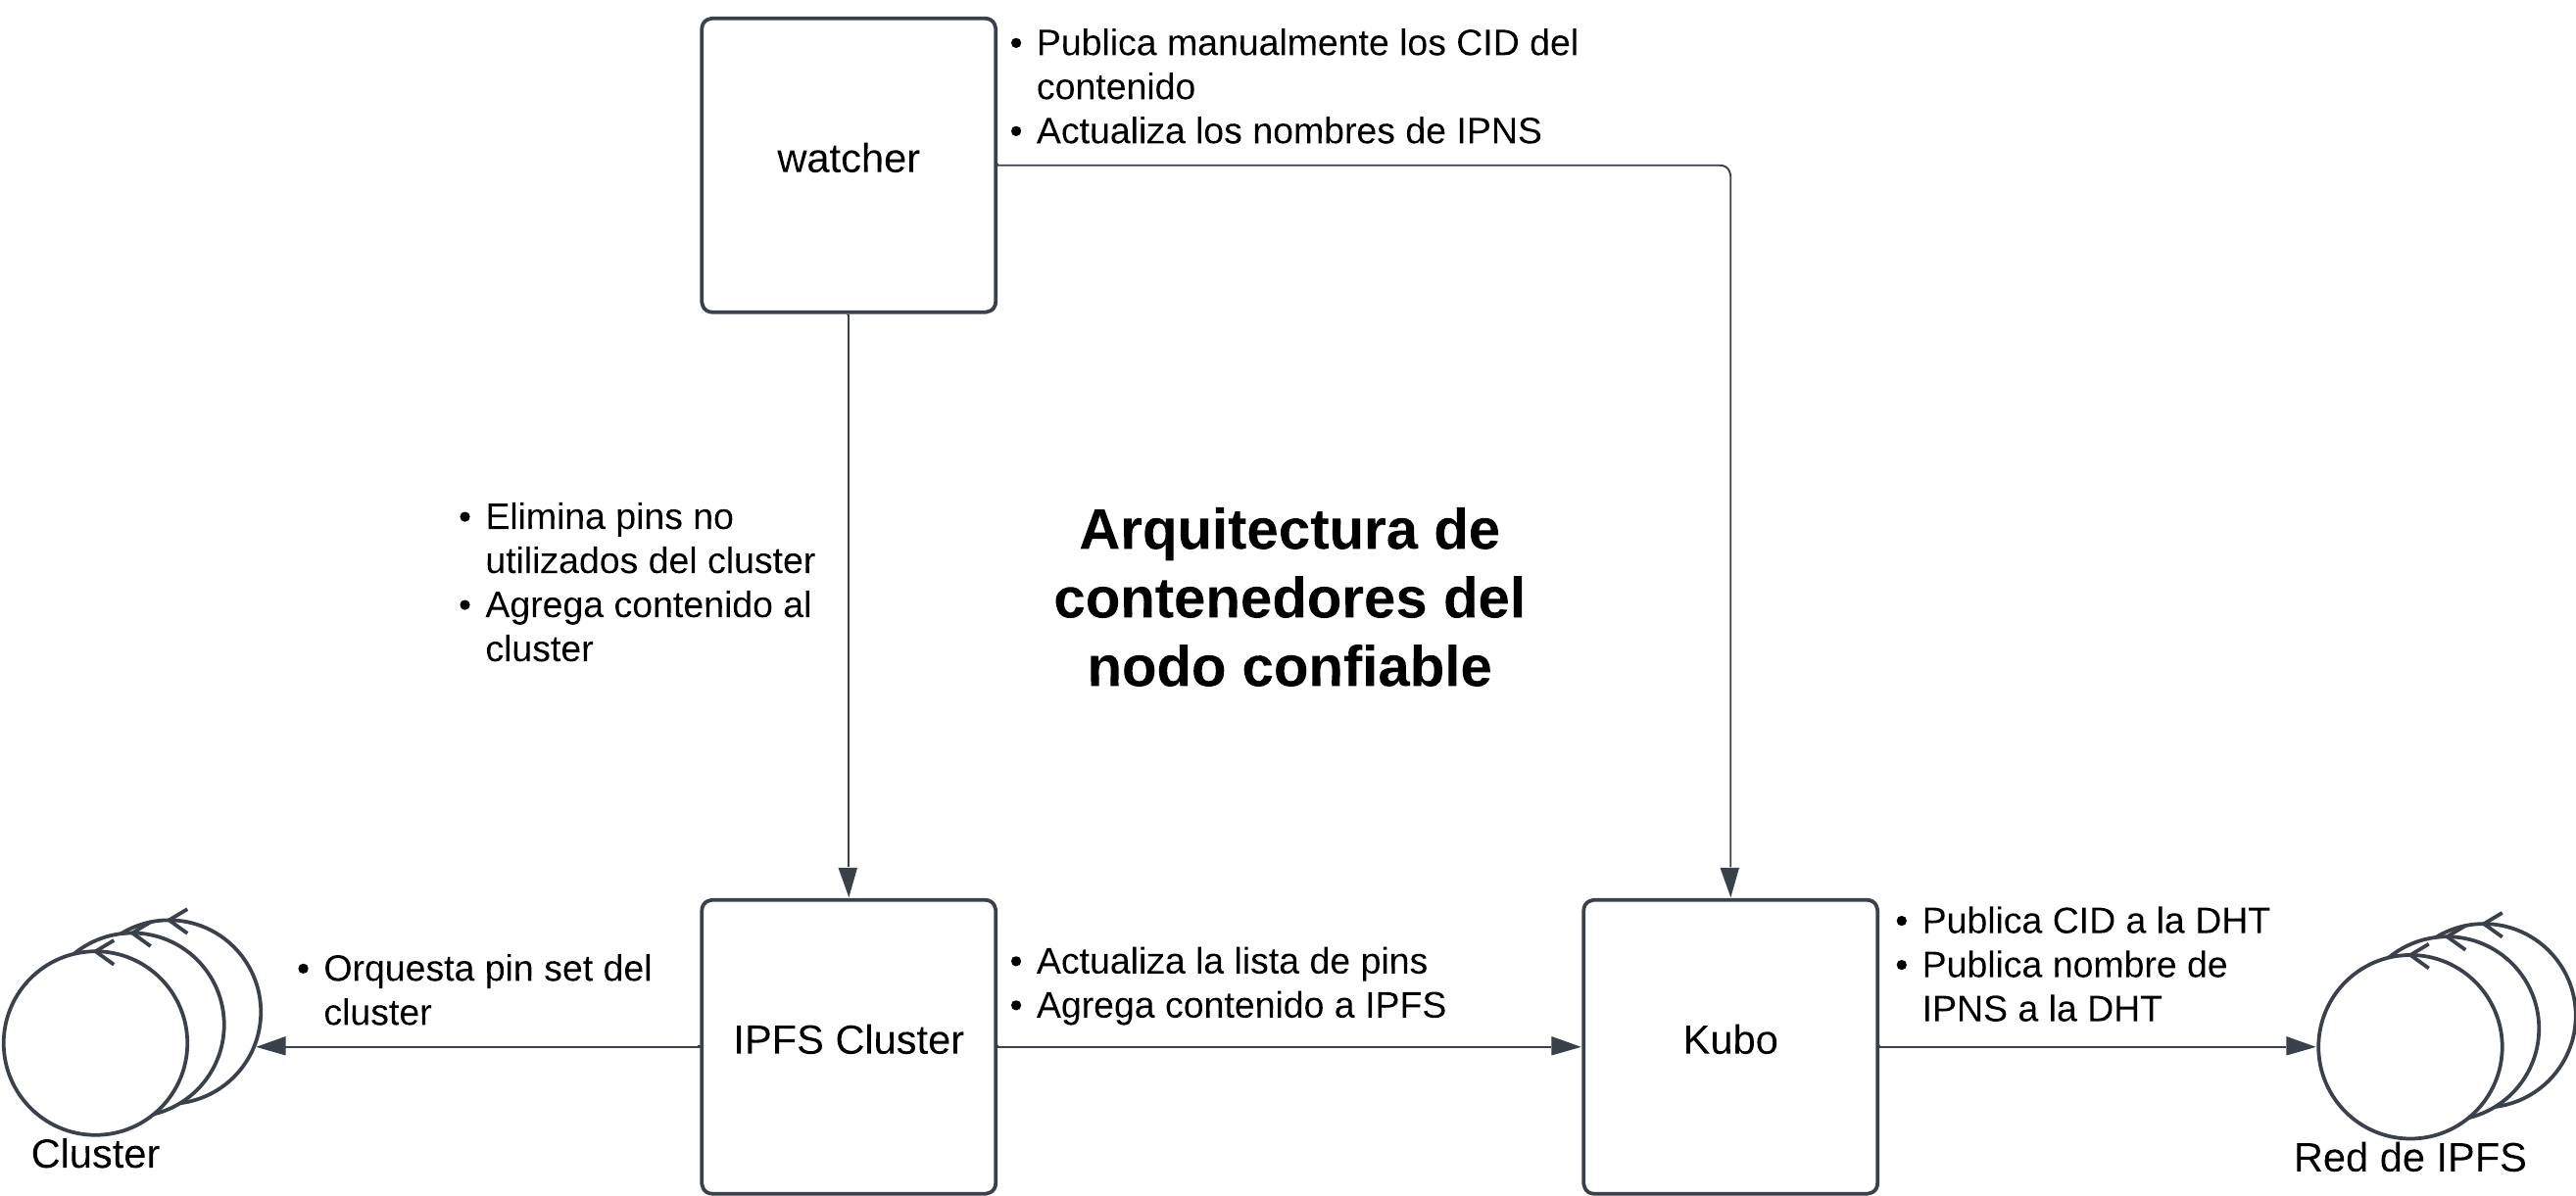
\includegraphics[width=1\linewidth]{img/solucion-ipfs/contenedores-trusted-peer.png}
    \caption{Mapa de interacciones entre los contenedores del nodo confiable}
    \label{fig:contenedores-trusted-peer}
\end{figure}

\subparagraph{Funcionamiento del Watcher} Este módulo del nodo confiable utiliza Git para comparar el último commit de la rama remota contra una copia local que se clona cada vez que se inicia. De esta manera, puede detectar cuando un nuevo cambio ocurre (tanto en el contenido como en \texttt{service.json}), e iniciar el proceso para obtener el nuevo cambio y desplegarlo. Dicho proceso se compone de los siguientes pasos:
\begin{enumerate}
    \item Subir el contenido y el \texttt{service.json} al Cluster, y obtener ambos CIDs.
    \item En base a los CIDs obtenidos, publicar ambos manualmente utilizando Kubo.
    \item Esperar a que todos los nodos dentro del cluster hayan pinneado los nuevos CIDs.
    \item Actualizar los dos nombres de IPNS para que apunten a los nuevos CIDs.
    \item Eliminar los pins antiguos del cluster.
\end{enumerate}

\begin{figure}[h!]
    \centering
    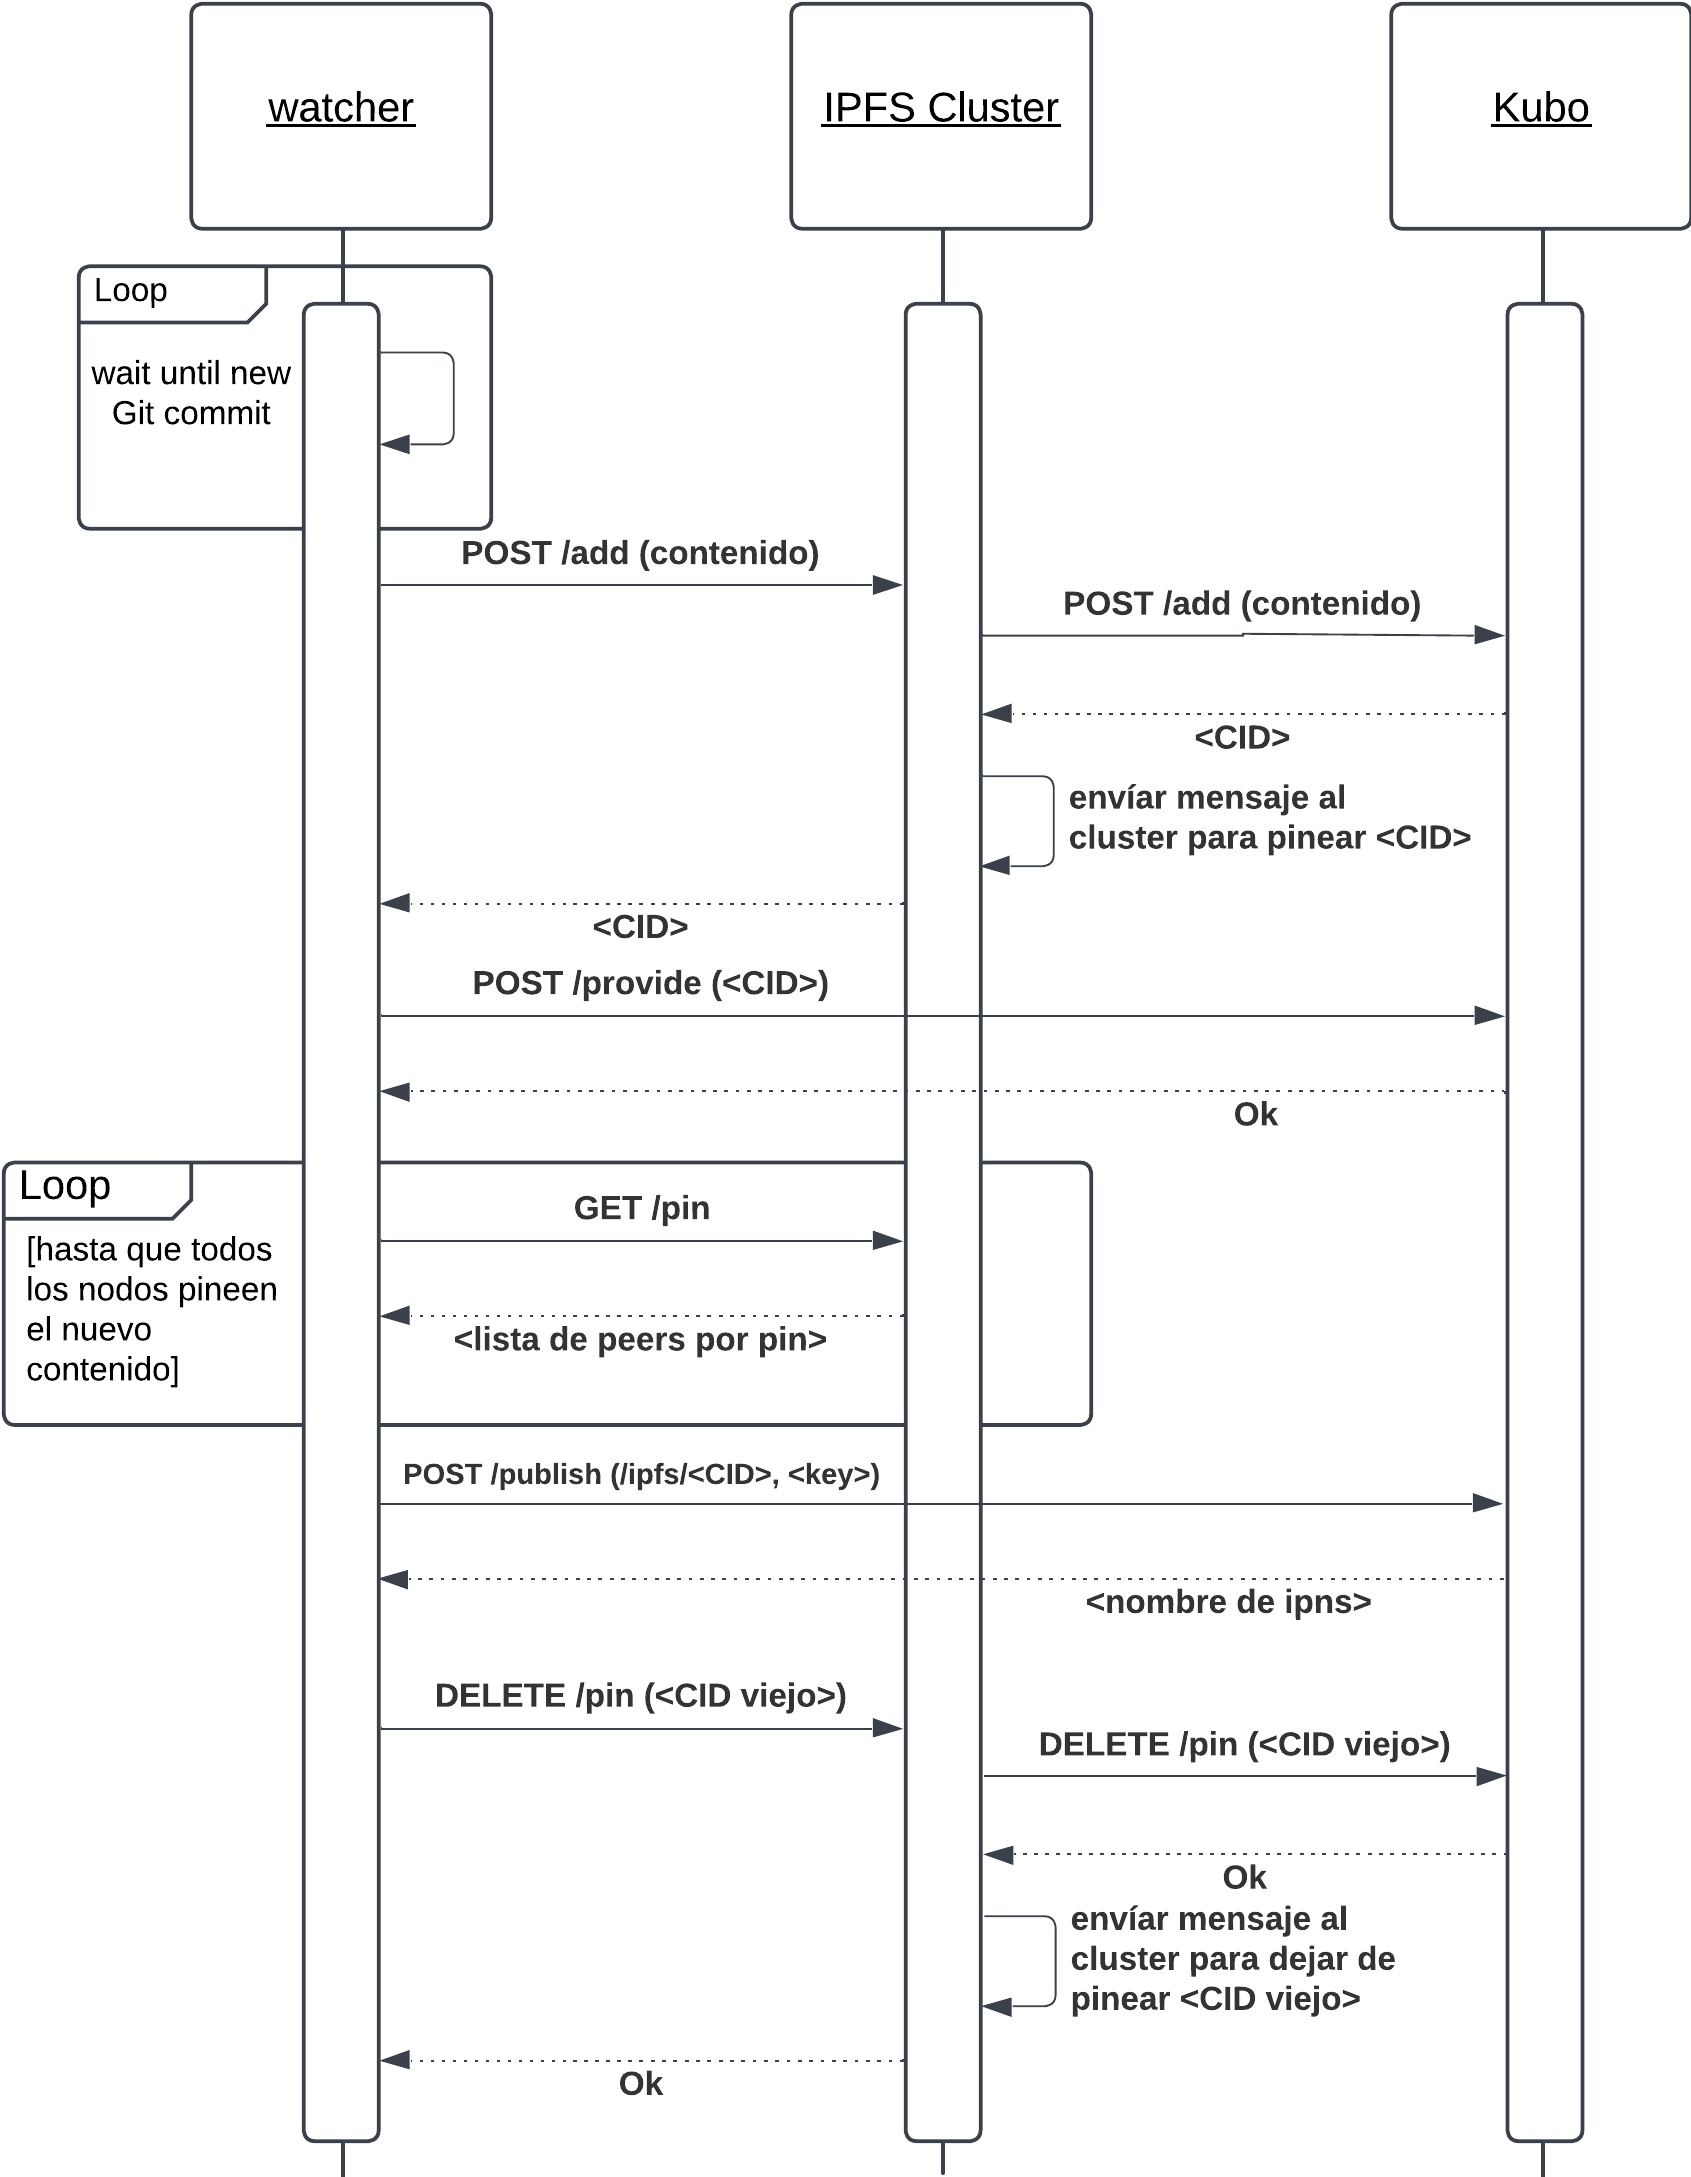
\includegraphics[width=0.5\linewidth]{img/solucion-ipfs/ds-trusted-peer.png}
    \caption{Diagrama de secuencia para el caso en que watcher detecta un cambio. Notar que para mayor claridad se omite los pasos para desplegar el nombre de IPNS del \texttt{service.json}, al ser exactamente los mismos que en el caso de un contenido.}
    \label{fig:contenedores-trusted-peer}
\end{figure}

\subparagraph{Disponibilidad} En el proceso mencionado para desplegar los cambios, existen dos factores que pueden afectar a la disponibilidad del contenido luego de recibir una actualización.

Por un lado, el nombre de IPNS puede no haberse actualizado en todos los nodos de la DHT, lo que provoca que algunos nodos apunten a la versión anterior del contenido. Esto se soluciona asegurándose de publicar el nuevo valor del nombre de IPNS \textbf{antes de instruir al cluster} para que deje de pinear la versión anterior.

Por otro lado, el contenido nuevo puede no estar disponible inmediatamente, ya que la publicación del CID en la DHT por parte del cluster se realiza de manera asíncrona. Para solucionar esto, se optó por publicar manualmente el CID con Kubo, de forma secuencial, antes de actualizar el nombre de IPNS. La desventaja de este enfoque es el tiempo adicional requerido para publicar el contenido, a cambio de garantizar su disponibilidad en todo momento, ya sea en su versión actual o en la nueva.

\subparagraph{Persistencia de la identidad del nodo}

Sabiendo que para ser un nodo confiable se debe tener su multiaddress en el archivo de \texttt{service.json}, es conveniente mantener el mismo PeerID a lo largo del tiempo y en distintas ejecuciones de la herramienta. Para ello, se debe indicar una \textit{identidad} que consiste de un PeerID, y una clave privada. Esto asegura que el nodo siempre se inicie con la misma identificación.

\subparagraph{Gestión de claves de IPNS}

Debido a la naturaleza de IPNS, un nombre solo puede ser modificado por un nodo que posea una clave privada determinada. Por ello, todos los nodos confiables deben tener las mismas clave privada de IPNS, una para el contenido y otra para \texttt{service.json}.

Para facilitar la inicialización, la herramienta provee un script que ayuda a generar la configuración y obtener los parámetros necesarios paso a paso. Esto incluye una identificación para el nodo, claves para IPNS, las direcciones de los repositorios de Git, y la IP pública necesaria para conectar los nodos a la red de IPFS.

\subparagraph{Integración con Git}

La manera en la que el contenedor \textit{watcher} puede detectar un cambio en el repositorio es consultando el repositorio remoto de Git cada minuto para identificar un cambio realizado y accionar el script de despliegue. Se requiere que el repositorio del contenido sea público, ya que la identificación por SSH o usuario y clave no están disponibles fácilmente dentro de un contenedor. De todas maneras, el contenido o archivos estáticos en el caso de una aplicación web ya son públicos por naturaleza, y debido al enfoque comunitario dado, que un repositorio necesite ser público no representa una restricción apreciable.

\subparagraph{Resultado}

La solución implementada logra automatizar el despliegue y la publicación de contenido en IPFS de forma confiable, simplificando muchos aspectos de IPFS y los clusters colaborativos. Mediante un comando \texttt{make up} se levanta un nodo confiable que automáticamente puede desplegar y mantener actualizado el contenido que se desee. Cabe destacar que, si bien el enfoque está diseñado para aplicaciones web, esta herramienta permite el despliegue de cualquier tipo de contenido, como repositorios, documentación, etcétera.

Combinando esta herramienta junto con un dominio ENS y un gateway con el cuál acceder al contenido, se obtiene una aplicación web cuyo uso es equiparable a la de un servidor HTTP moderno, sin diferencias perceptibles para el usuario, y de manera comunitaria, descentralizada, y económica.

\subsubsection{Infraestructura de aplicación}

Para aplicaciones que requieran mantener un estado y permitir que usuarios puedan modificarlo, no es suficiente con la infraestructura que explicamos anteriormente, ya que no hay una noción de estado y solo se le permite cambiar su contenido a los dueños de lo que se despliega. Es por eso que es necesaria otra infraestructura, la cual nos provea de esas necesidades.

Esta infraestructura surgió en base a un extenso desarrollo del cual nos ayudó a entender y encontrar la abstracción de lo que se estaba creando. Al principio del desarrollo, esta era gran parte de la arquitectura del primer caso de uso no estático que realizamos, el repositorio de conocimiento, para luego convertirse en una implementación propia, la cual llamamos \textbf{AstraDB}.

A continuación pasaremos a explicar cómo es la arquitectura que compone a AstraDB, cómo fue su evolución y que decisiones se tomaron a lo largo de su desarrollo, como también cómo podemos hacer uso de ella para fácilmente crear las aplicación que venimos a analizar, aplicaciones comunitarias, distribuidas y descentralizadas dentro del ecosistema de IPFS, tal como lo son el repositorio de conocimiento y el mensajero en tiempo real, las cuales hacen uso de AstraDB para su funcionamiento.

\paragraph{Etapa de investigación}

Al comenzar con el desarrollo del repositorio de conocimiento nos encontramos con un desafío, cómo podemos lograr que una aplicación dentro del ecosistema de IPFS pueda tener, modificar y guardar un estado.

Dada la naturaleza de IPFS, como explicamos anteriormente, no está pensado para alojar cambios en tiempo real. El modelo de direccionamiento por contenido implica que cualquier modificación genera un nuevo identificador (CID), lo que resulta inconveniente para actualizar un recurso directamente sin mecanismos adicionales. Por esta razón, utilizar únicamente el conjunto de protocolos que IPFS ofrece no nos resulta conveniente para aplicaciones dinámicas.

Como sucede con un caso de uso muy similar al repositorio de conocimiento que queremos implementar, el proyecto de \textbf{Distributed Wikipedia Mirror}\cite{distributed-wikipedia-mirror}, el cual consistió en poner una versión de wikipedia en IPFS, únicamente funciona como versión Read-Only, y con snapshots manuales, lo cual es totalmente posible de hacer con la infraestructura que explicamos anteriormente.

Es por esto que resulta de un verdadero desafío lograr que una versión Read-Write sea posible sin sacrificar los principios de decentralización que IPFS nos provee. Para abordar esta limitación nos llevó a buscar herramientas complementarias dentro del ecosistema y ahí fue cuando nos encontramos con \textbf{OrbitDB}\cite{orbitdb}.

\paragraph{Representación de los datos}

OrbitDB es una base de datos peer-to-peer, distribuida y sin un servidor central. Utiliza IPFS para el almacenamiento de datos y \textbf{Libp2p}\cite{libp2p} para sincronizar automáticamente las bases de datos con otros peers. Es una base de datos \textbf{eventualmente consistente} que utiliza Merkle-CRDTs para escrituras y fusiones de base de datos libres de conflictos, lo que hace que OrbitDB sea una excelente opción para aplicaciones p2p y descentralizadas.
% , y en nuestro caso, para una wiki decentralizada.

OrbitDB ofrece varios tipos de bases de datos para diferentes modelos de datos y casos de uso. Algunos que se asemejan más a bases de datos convencionales, como puede ser un simple key-value y otros más distintos como puede ser uno de eventos secuenciales.

Uno de los requisitos de la infraestructura desarrollada es lograr una verdadera descentralización, significando que no haya una entidad o persona con mayores permisos sobre el resto, esto se traduce, en parte, a permitir que cualquiera que quiera pueda crear y/o modificar la base de datos sin ninguna restricción. Para lograr esto, OrbitDB nos permite indicar que cualquier nodo tenga permiso de edición sobre una base de datos. El problema es que esto también permitiría que cualquier usuario pueda eliminar información de la base de datos y es algo que no nos podemos permitir y es esta la principal razón por la cual no podemos utilizar un tipo como key-value, o documentos y necesitamos otro que se adecúe más a nuestro caso.
 
OrbitDB nos provee de otro tipo de base de datos, el tipo de events. Un tipo de base de datos el cual es inmutable (append-only), un log transversal que muestra un historial que se puede recorrer. Sin embargo surgen nuevos desafíos.

Gracias a que es un tipo append-only ya no se tiene el problema de posible perdida de información, ya que un usuario solo puede agregar un nuevo valor a la base de datos y no eliminar valores agregados previamente, sin embargo nos surge otro problema, como representamos la información con una base de datos que solo se puede agregar?

La solución es separarnos de la idea de que se tiene que tener una única base de datos que albergue toda la información. Al pensarlo desde el punto de vista del repositorio de reconocimiento, podemos representar cada articulo como su única base de datos de eventos y cada valor que se le agrega puede ser el cambio que se le hizo al articulo y al leer su historia se puede reconstruir a su última versión.. Esto resulta de una práctica muy común en estas arquitecturas distribuidas.

\begin{figure}[h!]
    \centering
    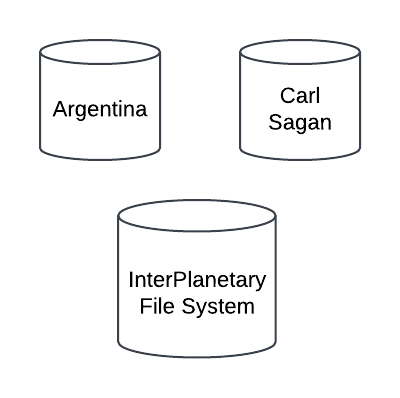
\includegraphics[width=0.5\linewidth]{img/solucion-ipfs/bdd-articulos.png}
    \caption{Representación de cada articulo como su propia base de datos.}
    \label{fig:bdd-articulos}
\end{figure}

De esta manera ya tenemos una representación para los artículos, pero faltaría una forma de saber que artículos existen actualmente. Es por eso que tenemos que agregar una última base de datos, también de eventos, que represente la wiki en si, con los nombres de los artículos existentes. De esta manera un usuario puede saber, al acceder a esta base de datos representando un repositorio de artículos, cuales son los artículos que existen y solo acceder a la base de datos correspondiente a ese articulo, sin necesidad de replicar la totalidad de los artículos existentes, algo que sería inviable.

\begin{figure}[h!]
    \centering
    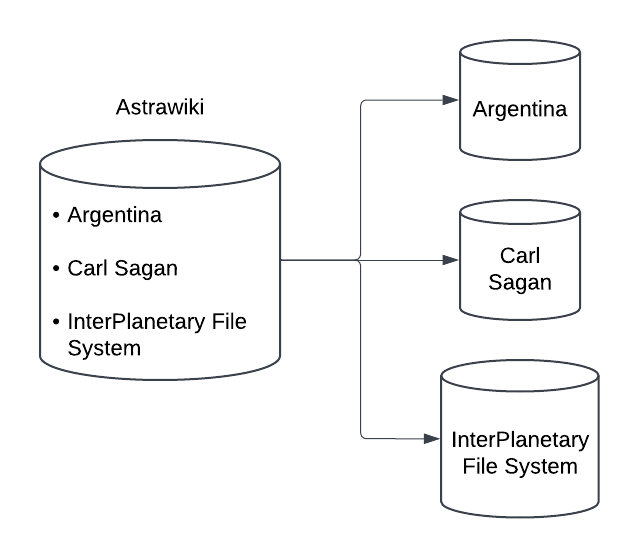
\includegraphics[width=0.5\linewidth]{img/solucion-ipfs/bdd-wiki.png}
    \caption{Representación de la base de datos de la wiki.}
    \label{fig:bdd-wiki}
\end{figure}

Ahora bien, como podemos acceder a la base de datos. En OrbitDB las bases de datos tienen una dirección que las identifica, formada en su creación. Esta dirección está conformada por el nombre de la base de datos, su tipo y su \textit{Access Controller}. Este último sirve para indicar quien tiene acceso y permisos sobre la base de datos. Como en nuestro caso estamos permitiendo que todos tengan permiso, el controller va a ser siempre el mismo. Esto nos es importante, ya que significa que al crear la base de datos siempre vamos a tener una misma dirección y es por eso que con solo saber el nombre de un articulo podemos saber la dirección de la base de datos que la compone, no necesitamos guardarnos ninguna dirección especifica. Lo mismo sucede con la base de datos representando la wiki, con saber el nombre de la wiki podemos acceder a ella.

\begin{figure}[h]
\centering
\fbox{\texttt{/orbitdb/zdpuAmrcSRUhkQcnRQ6p4bphs7DJWGBkqczSGFYynX6moTcDL}}
\caption{Ejemplo de un \textit{address} de una base de datos de OrbitDB.}
\end{figure}

\paragraph{Colaboradores}

En orbitdb, al ser una base de datos peer-to-peer, distribuida y sin un servidor central, significa que la base de datos existe en cada peer que la componga, por lo tanto conectarse a una base de datos significa replicar la totalidad de su información de otros peers que nos la provean. De no estar esos peers, significaría que la base de datos no puede ser accedida y su información podría perderse, tal como sucedía cuando explicamos la infraestructura anterior. Es por eso que una gran parte de la arquitectura está pensada al rededor de peers que opten por ser colaboradores, estos peers van a replicar todas las bases de datos que existan actualmente en la base de datos central, pensandolo en el caso del repositorio, van a preservar todos los articulos que existan. De esta manera logramos que mientras haya por lo menos un colaborador en linea, la wiki va a poder ser accedida.

Estos peers colaboradores son el punto más importante que diferencia esta solución con el resto y que sigue con la filosofía de las aplicaciones comunitarias que estamos analizando, permitiendo que la disponibilidad de la información se este logrando a traves de la donación de almacenamiento en vez de dinero.

\paragraph{Manejo de conexión}

Entonces, un usuario que quiera conectarse a la base de datos y obtener su información, por ejemplo querer conectarse a la wiki y ver artículos, debe primero conectarse a alguno de estos colaboradores, de los cuales puede replicar la información a su base de datos propia.

OrbitDB no se responsabiliza de manejar las conexiones, tampoco le importa, ya que te asegura que eventualmente la base de datos va a estar sincronizada entre peers, aunque se caigan las conexiones o te conectes mas tarde, todo se va a sincronizar sin conflictos. Por lo tanto delega esa responsabilidad a \textbf{Helia}\cite{helia} la cual es la implementación de IPFS en los lenguajes javascript/typescript, que a su vez delega la responsabilidad a \textbf{LibP2P}\cite{libp2p} y de la cual tenemos que hacer uso nosotros para manejar las conexiones.

LibP2P es una colección de protocolos y utilidades para facilitar la implementación de una red peer-to-peer. 
Al crear un nodo de LibP2P se tiene que elegir como conformarlo en base a un conjunto modular de herramientas,
dentro de los que se encuentran mecanismos de seguridad, de transporte, descubrimiento de pares, entre otros. Cada una de estas herramientas es importante y hace que el nodo funcione como queramos, más adelante explicaremos la decisión para cada herramienta elegida, sin embargo ahora nos vamos a centrar en dos protocolos de interés necesarios para solucionar el problema de manejo de conexión. Los protocolos de transporte y de descubrimiento de peers.

Los protocolos de transporte son los encargados de la comunicación entre nodos, de manera similar a la capa de transporte presente en toda red convencional. Se basan en tipos de transporte ya existentes, adaptados al uso peer-to-peer. Como son TCP, WebSockets, entre otros.








Colección de protocolos y utilidades para facilitar la implementación de una red peer-to-peer \cite{libp2p}. Entre sus herramientas, se encuentran diferentes mecanismos de seguridad, de transporte, y para descubrimiento de pares. Se creó con IPFS en mente, pero luego se expandió a un conjunto de protocolos independiente, el cual es utilizado por Ethereum actualmente. Los protocolos de interés para este proyecto son:
\subparagraph{Protocolos de transporte} Son los encargados de la comunicación entre nodos, de manera similar a la capa de transporte presente en toda red convencional. Se basan en tipos de transporte ya existentes, adaptados al uso peer-to-peer. Los protocolos principales son TCP, WebSockets y WebRTCDirect.
\subparagraph{Protocolos de descubrimiento de peers} Para encontrar un contenido en IPFS, se necesita saber la dirección del nodo que tiene dicho contenido. El principal protocolo para lograr esto se denomina Distributed Hash Table (DHT) \cite{dht}. Es un registro clave-valor distribuido en todos los nodos que soporten este protocolo, que contiene la información necesaria para encontrar el contenido deseado. Cada nodo tiene una parte de esta tabla, y deberá preguntar a otros nodos hasta conseguir la dirección del nodo asociada a la dirección del contenido buscado.



\paragraph{AstraDB}

Para entender cómo funciona AstraDB, primero entendamos resumidamente qué es.

AstraDB es una abstracción de una base de datos "key-value like" orientada para aplicaciones comunitarias en el ecosistema de IPFS. Es una base de datos descentralizada y distribuída, peer-to-peer, la cual hace uso de tecnologías como \textbf{OrbitDB} \cite{orbitdb} para el manejo de datos y \textbf{LibP2P} \cite{libp2p} para la comunicación peer-to-peer entre usuarios.

Su arquitectura tiene 2 grandes responsabilidades. Por un lado tiene que encargarse del manejo de lo datos, permitir que la aplicación tenga un estado y este pueda ser modificado por parte de cualquier usuario. Por otro lado debe proveer la forma de conectar y proveer de información a los distintos usuarios, para que estos puedan comunicarse y notificarse de nuevos cambios.

\paragraph{Manejo de los datos}

% Sin embargo en ningún momento vamos a estar abriendo explícitamente una base de datos con esa dirección, sino que vamos a estar creando la misma base de datos vacia desde cero y sincronizandola con el resto. Esto sucede ya que, si recordamos, orbitdb es una base de datos \textbf{eventualmente consistente} esto significa que orbitdb te asegura que en algún momento todas los nodos van a tener la misma información, pero no tenes certeza de cuando va a suceder. Es por esto que desde la arquitectura se toman ciertos recaudos teniendo en cuenta esto, y es por eso que no podemos nunca estar seguros si somos los primeros en crear una base de datos o ya existe y aun no fuimos sincronizos, generando como un chicken-egg problem
\subsection{Blockchain}

En este trabajo se utilizó la red de Ethereum, al ser una blockchain popular nos permite demostrar y comparar los casos de uso contra nuestra solución en IPFS. Ethereum está compuesta de nodos distribuidos que comparten poder de cómputo lo cual permite el desarrollo de aplicaciones descentralizadas. Cuenta con una moneda que funciona a modo de incentivo, es decir, que los nodos reciben ganancias por formar parte de la red. Esto conlleva a que los usuarios de la red necesiten pagar para utilizarla a través de transacciones.

\subsubsection{Swarm}

Para el desarrollo del sitio web estático se decidió ir por Swarm que es un almacenamiento descentralizado que corre sobre una \textit{sidechain} de Ethereum. Swarm surgió como uno de los tres pilares de Ethereum para una web descentralizada \parencite{swarm-origin}. Funciona por \textit{content addressing} como IPFS e incluye un modelo de incentivos utilizando su propia moneda llamada BZZ.

\paragraph{Feed}

Los \textit{feeds} en Swarm funcionan de manera similar a los IPNS de IPFS. Es un puntero, con CID fijo, a un archivo. Esto permite actualizar el archivo al que apunta un \textit{feed} manteniendo un punto de entrada fijo al sitio web.

\subsubsection{Ethereum}

Para los casos de uso del repositorio de conocimiento y el mensajero en tiempo real necesitamos una herramienta que nos funcione de manera \textit{read-write} y como Swarm solamente se encarga de archivos estáticos buscamos alguna alternativa dentro del ecosistema blockchain. Para esto terminamos usando Ethereum.

\begin{figure}[H]
    \centering
    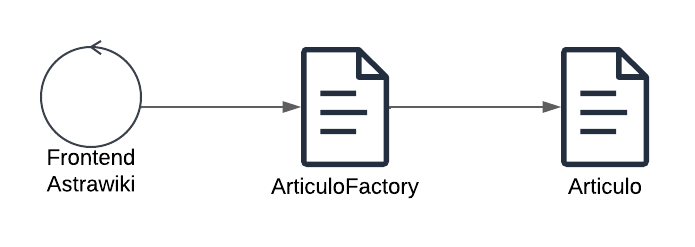
\includegraphics[width=0.5\linewidth]{img/astrawiki-articulo-factory.png}
    \caption{\textit{Smart contracts} que intervienen en el repositorio de conocimiento}
    \label{fig:aw-eth-articulo-factory}
\end{figure}

Ambos casos de uso resultaron muy similares en su resolución, haciendo uso del patrón de diseño \textit{Factory}. Existe un smart contract Factory que crea otros smart contracts (Artículo o Chat, según el caso de uso).

\begin{figure}[H]
    \centering
    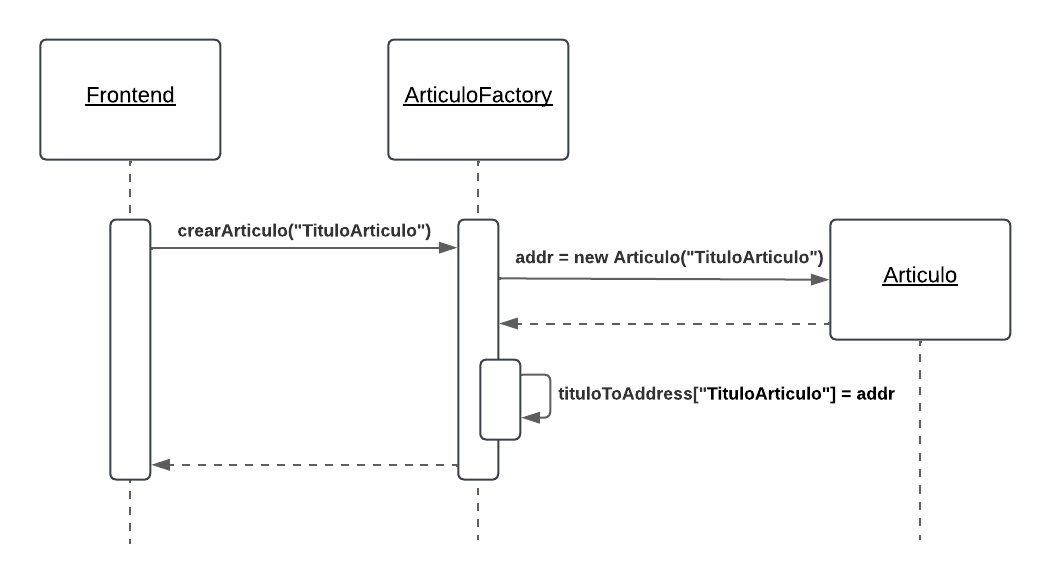
\includegraphics[width=0.75\linewidth]{img/ds-aw-eth-crear-articulo.png}
    \caption{Creación de un artículo}
    \label{fig:ds-aw-eth-crear-articulo}
\end{figure}

De esta manera el \textit{Factory} tiene un \textit{mapping} con todos los artículos creados y las direcciones correspondientes para accederlos. Si se quisiera acceder a un Artículo en particular primero se tiene que consultar al \textit{Factory} para obtener la dirección del mismo y, como cada artículo es un \textit{smart contract} en sí mismo, se puede consultar o modificar su contenido directamente interactuando con el Artículo en particular como se puede ver en la Figura \ref{fig:ds-aw-eth-obtener-contenido-articulo}.

\begin{figure}[H]
    \centering
    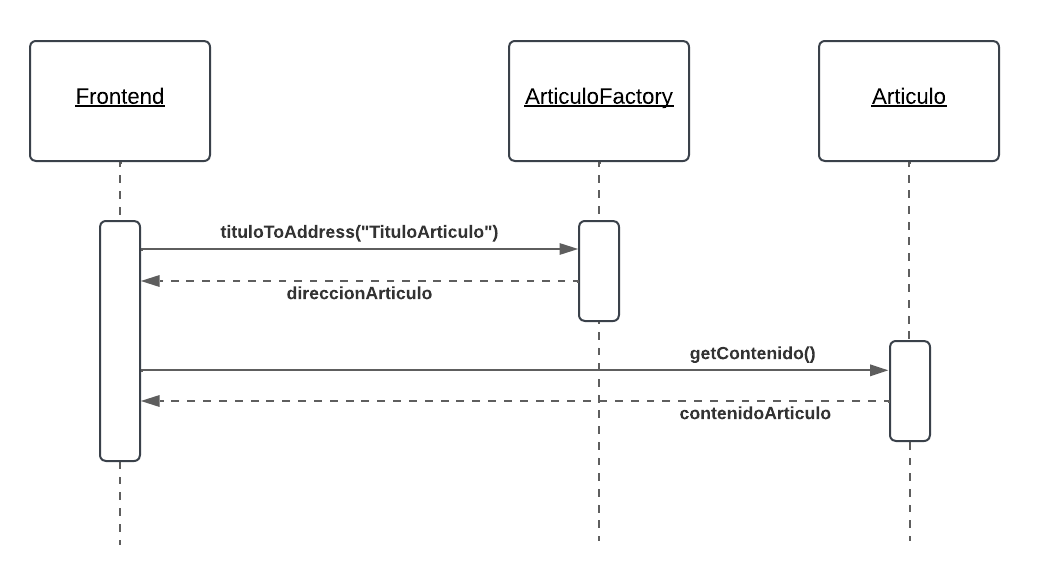
\includegraphics[width=0.75\linewidth]{img/ds-aw-eth-obtener-contenido-articulo.png}
    \caption{Obtención del contenido de un artículo}
    \label{fig:ds-aw-eth-obtener-contenido-articulo}
\end{figure}

La principal diferencia entre el repositorio de conocimiento y el mensajero en tiempo real está en que los mensajes del mensajero tienen que ser vistos por los demás usuarios que participan de la conversación en el momento que se envían. Esto no es estrictamente necesario en el repositorio de conocimiento pero sí lo es en el mensajero.

Para afrontar este requisito se utilizaron los eventos de Solidity (el lenguaje de programación en el que se desarrollan los \textit{smart contract} de Ethereum). Funciona de la siguiente manera, al momento de enviar un mensaje se emite un evento. Este evento se recibe en un listener que fue previamente inicializado al instante previo de haber obtenido el Chat en el frontend. Al recibir este evento el frontend puede actualizar la pantalla mostrando el mensaje nuevo sin necesidad de obtener todos los mensajes.

% TODO: insertar gráfico del flujo de un evento al enviar un mensaje 

Por otro lado, para el mensajero en tiempo real necesitamos una manera de identificar a cada usuario. Para esto se hizo uso de las \textit{wallets}. Cada usuario se identifica utilizando su \textit{wallet}, que tiene una clave pública, que pasa a ser el identificador del usuario, y una clave privada la cuál es necesaria para firmar transacciones en nombre del usuario, que en nuestro caso funciona a modo de contraseña. Además, para que la lectura de las conversaciones sean más usables, se agregó la posibilidad de generar un nombre de usuario asociado al identificador del mismo. A este nombre de usuario lo llamamos alias y es único para todos los Chats asociados a un mismo ChatFactory. Una vez el usuario se conecta con su \textit{wallet}, puede elegir un alias y cambiarlo cuando desee siempre y cuando no exista actualmente algún otro usuario con ese mismo alias.

Finalmente, nos queda la funcionalidad de que un usuario pueda responder a otro mensaje. Primero necesitamos una manera de identificar a cada mensaje de manera unívoca. El identificador de cada mensaje se genera hasheando el timestamp del bloque, el identificador del emisor y la cantidad de mensajes en el chat en el momento que se envía. Luego, cuando se responde a otro mensaje se almacena el identificador del mensaje al que se está respondiendo (el mensaje padre) dentro de la estructura del mensaje que se está enviando. Todo esto se resuelve dentro del \textit{smart contract} del Chat correspondiente.


% \newpage

\subsection{Front-end}

% TODO: Mostrar un diagrama de cómo todos los paquetes de bitxenia se utilizan y interactuan entre sí para que el front-end los termine usando. 

Como prueba de la versatilidad de los ecosistemas, y aprovechando la creación de paquetes, se desarrollaron diferentes front-ends para las aplicaciones realizadas.

\paragraph{Astraweb}

El principal front-end que contiene el repositorio de conocimiento y a su vez el mensajero en tiempo real. Además, posee la opción de escoger el ecosistema al que se desea conectar.

\begin{figure}[H]
    \centering
    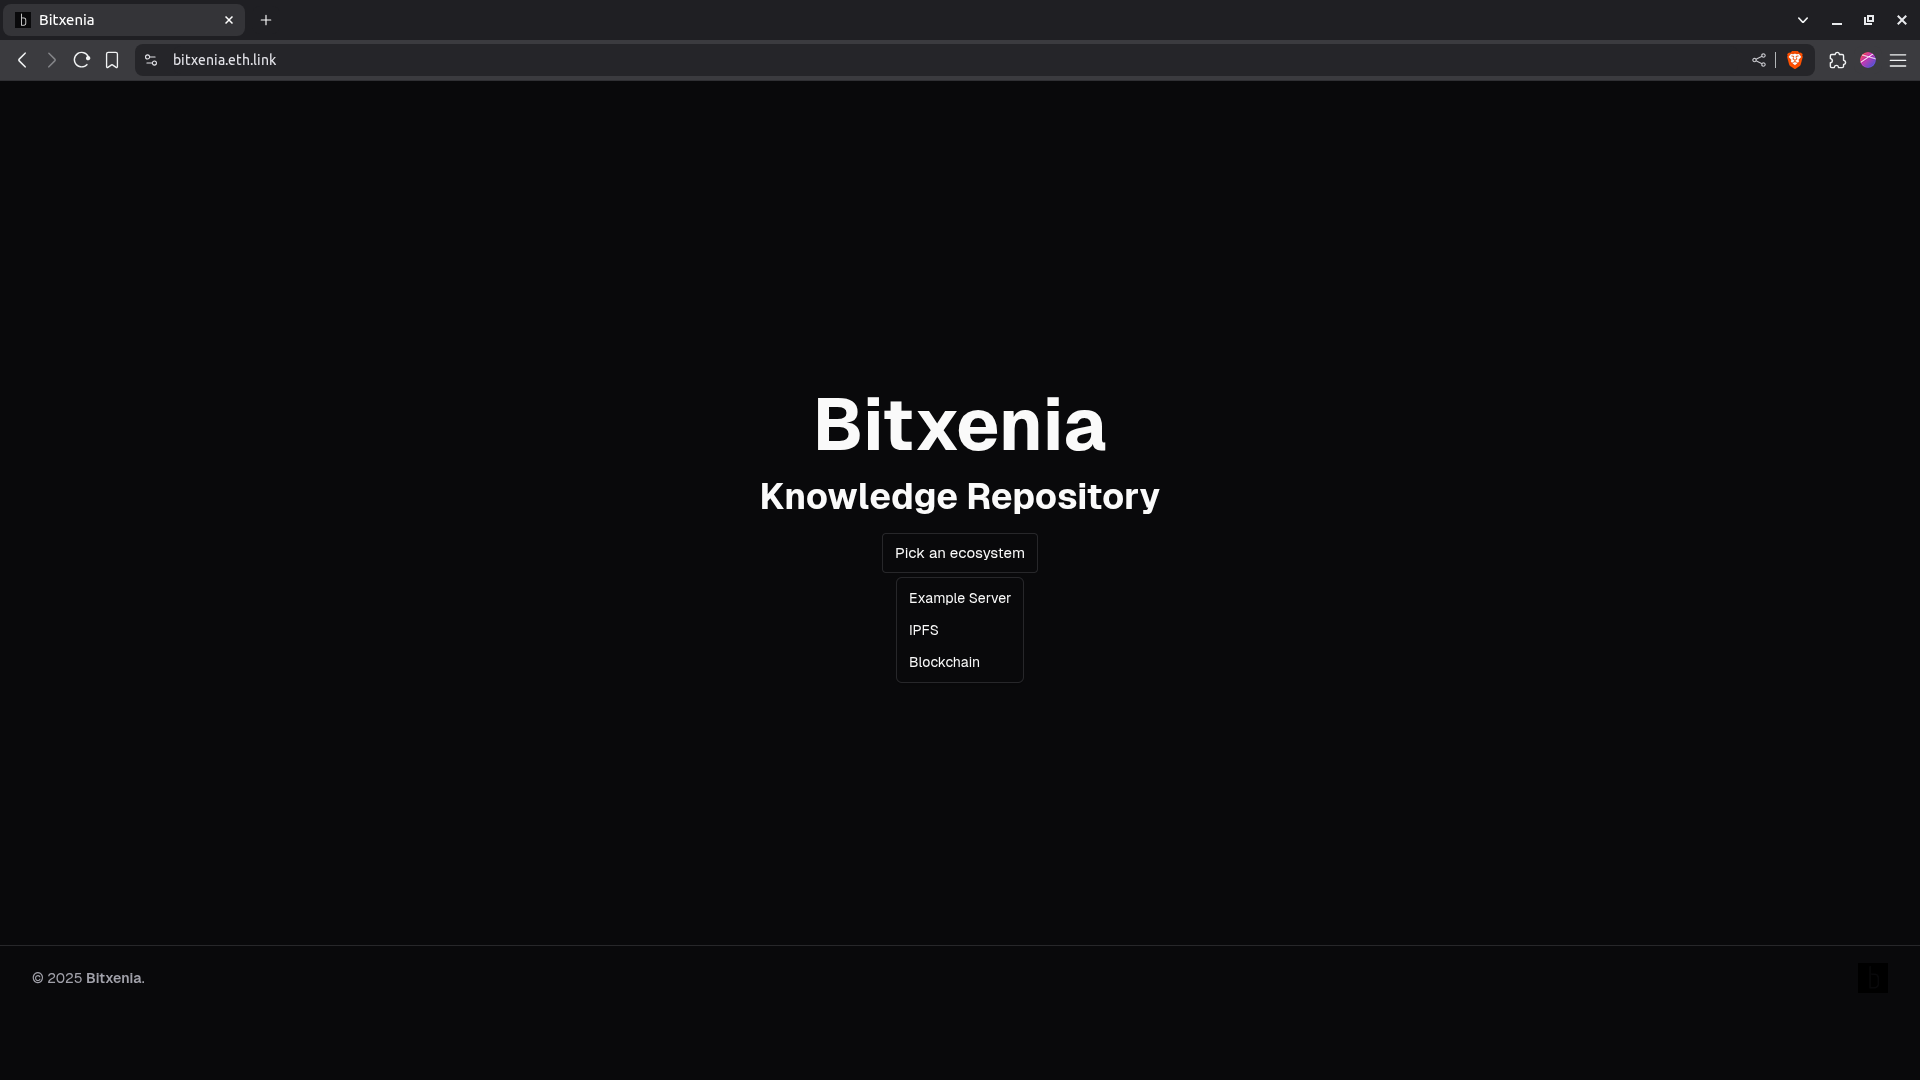
\includegraphics[width=1\linewidth]{img/astraweb-main-page.png}
    \caption{Página principal de Astraweb}
    \label{fig:astraweb-main-page}
\end{figure}

\subparagraph{Tecnología} Se utilizó \texttt{React} \cite{react} y \texttt{Next.js} \cite{next} como \textit{frameworks} para la creación de la aplicación web, basándonos en una plantilla llamada \texttt{rubix-documents} \cite{rubix}. El código fue escrito en \texttt{Typescript}.

\subparagraph{Servidor ejemplo} Se desarrolló una solución centralizada como tercer ecosistema para este frontend, con dos propósitos:
\begin{enumerate}
    \item Paralelizar el desarrollo del front-end y los distintos paquetes de cada ecosistema. Debido a que se definió una interfaz común tanto para el repositorio de conocimiento como para el mensajero en tiempo real, se logró avanzar con el front-end haciendo pruebas manuales con este servidor.
    \item Comparar las implementaciones descentralizadas contra un enfoque centralizado.
\end{enumerate}
El servidor fue creado en \texttt{Node.js} con \texttt{Express.js} como framework para interactuar con \textit{requests} de HTTP.

\subparagraph{Limitaciones} Debido a la falta de un servidor tradicional para ofrecer el contenido, el uso de \textit{Server Components} o componentes de servidor \cite{server-components} no era posible. Esto implicó modificar ampliamente la plantilla utilizada para descartar este tipo de componentes en favor de aquellos que pueden ser compilados y luego utilizados por el cliente sin interacción con un servidor.

\paragraph{Astrawiki CLI}

Front-end de terminal, desarrollado para el caso de uso del repositorio de conocimiento y para el ecosistema de IPFS en específico. Cuenta con todas las funcionalidades del repositorio de conocimiento, como crear, editar y ver artículos, consultar versiones pasadas, e incluso colaborar, lo cual se verá en el apartado de IPFS. Además, cuenta con un contenedor \texttt{Docker} publicado, con el fin de fácilmente iniciar un nodo sin necesitar una instalación de \texttt{Node} y demás dependencias. Funciona como un \texttt{daemon} \cite{daemon}, es decir, se inicia y funciona en segundo plano hasta que se indique lo contrario.

Su propósito es, por un lado demostrar la versatilidad del modelo de paquetes utilizado para crear distintos front-ends. Y por otro lado, el contenedor es útil para el nodo colaborador desarrollado para IPFS, el cual se basa en diferentes contenedores y se verá más adelante.

\subparagraph{Arquitectura} Se compone de un cliente, el cuál se inicia con cada comando (\texttt{start}, \texttt{add}, \texttt{get}, \texttt{edit}, \texttt{list}, etc.) y un servidor que se ejecuta por detrás, el cual inicia la instancia del repositorio de conocimiento de IPFS y utiliza su API cuando recibe \texttt{requests HTTP}.

\begin{figure}[H]
    \centering
    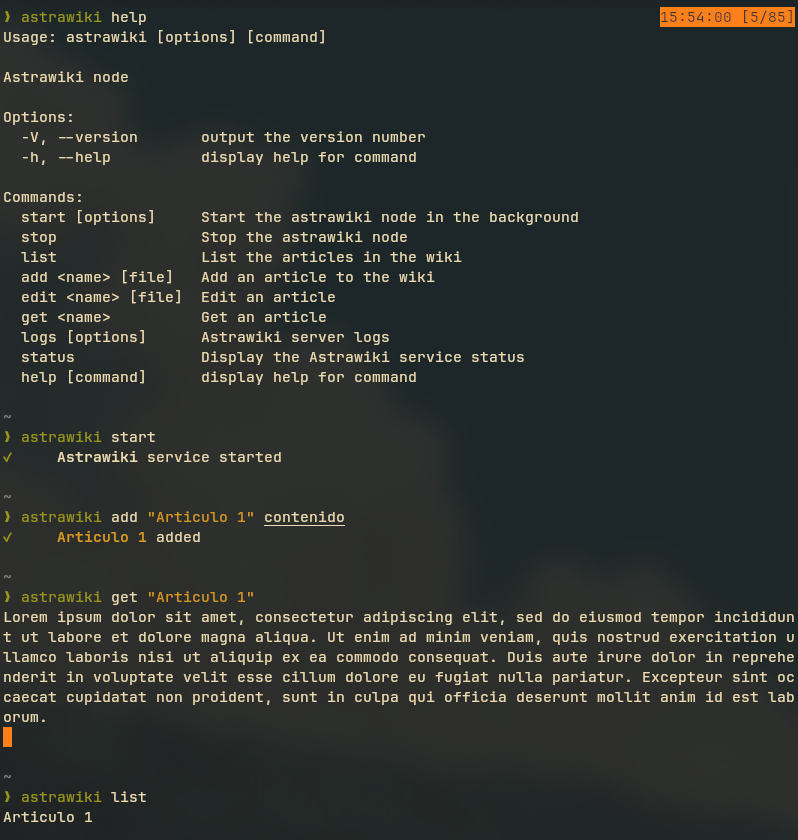
\includegraphics[width=0.7\linewidth]{img/astrawiki-cli.png}
    \caption{Ejemplo de uso de \texttt{astrawiki-cli}}
    \label{fig:astrawiki-cli}
\end{figure}

% TODO: Agregar imágenes de la terminal con ejecuciones de astrawiki-cli.

\paragraph{Astrachat CLI}

Frontend de terminal, desarrollado para el caso de uso de mensajero en tiempo real y para el ecosistema de Blockchain.

\begin{figure}[H]
    \centering
    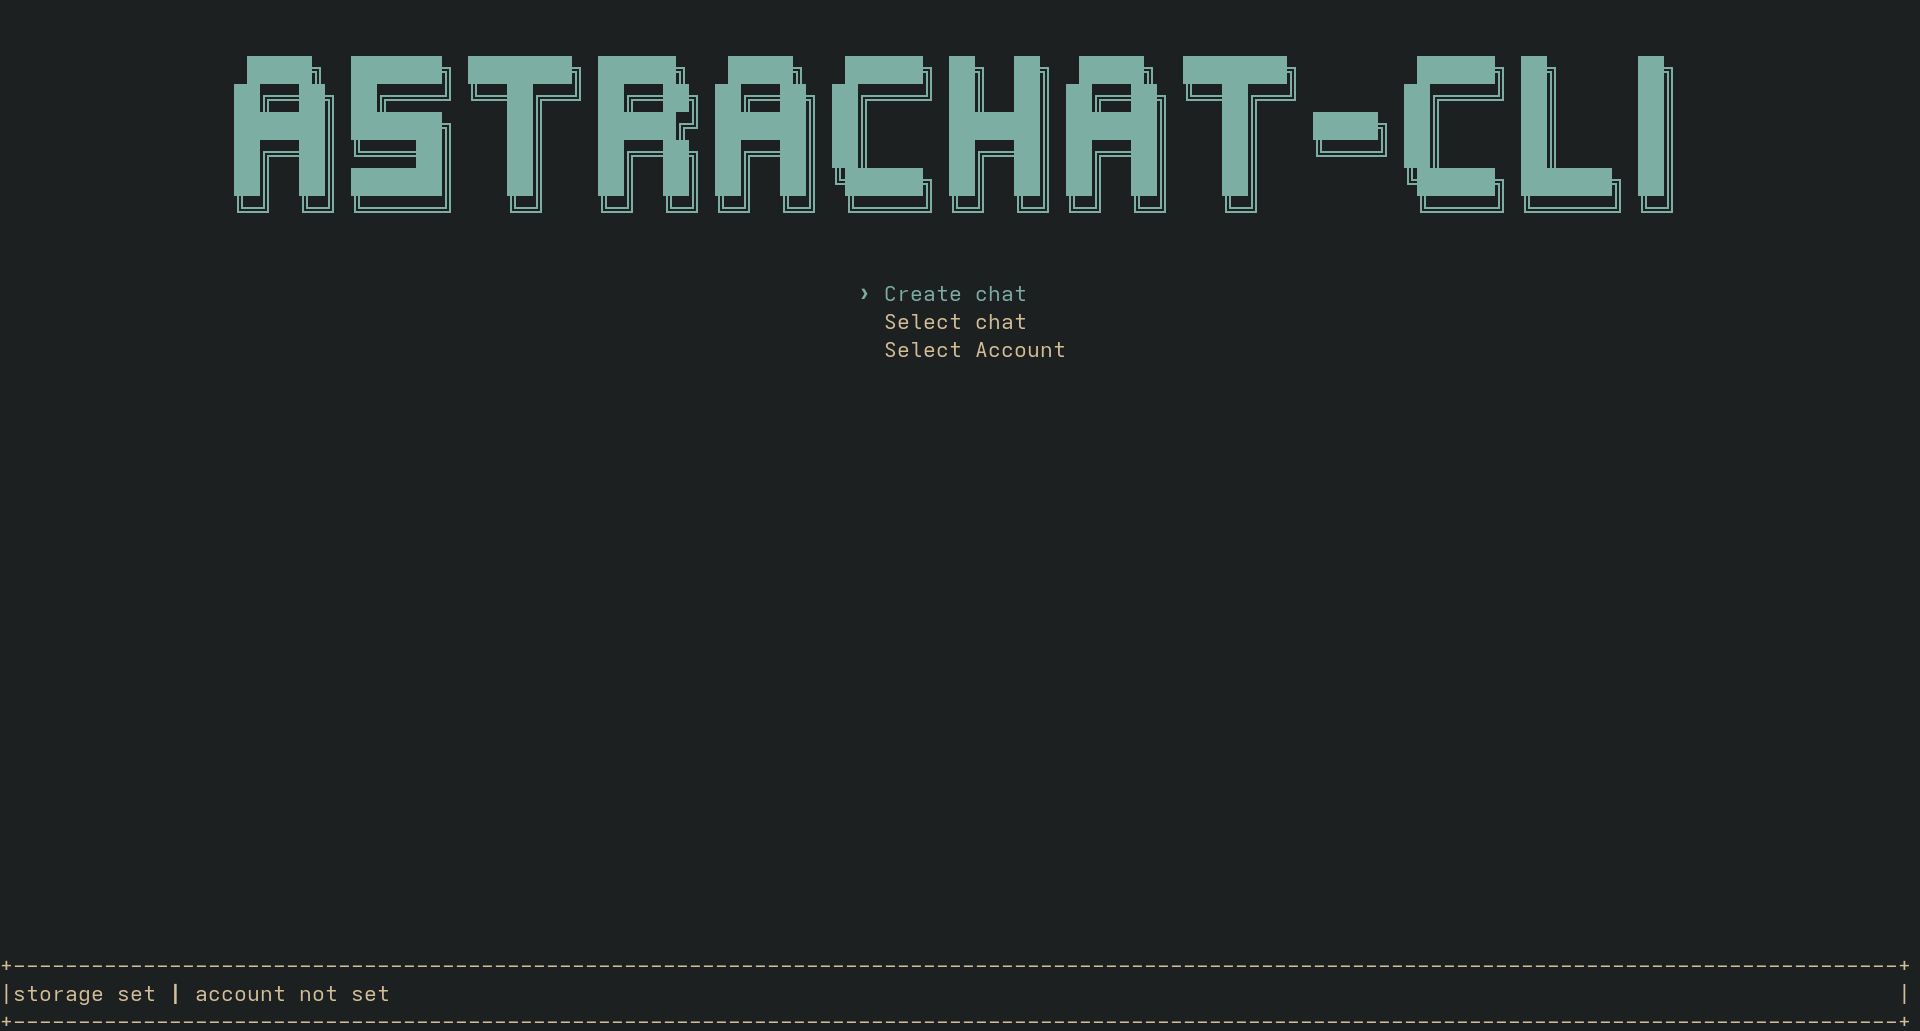
\includegraphics[width=1\linewidth]{img/astrachat-cli-main-page.png}
    \caption{Página principal de \texttt{astrachat-cli}}
    \label{fig:astrachat-cli-main-page}
\end{figure}
\section{Metodología aplicada}

La metodología aplicada para la gestión del proyecto fue una versión aproximada a Scrum. El desarrollo se dividió en sprints semanales para los cuales utilizamos un tablero Kanban en Github Projects donde se fueron agregando las tareas a realizar para cada caso de uso y ecosistema. Se realizaron reuniones semanales fijas que se usaron como punto de control, donde se revisó lo hecho durante la semana y definimos pasos a seguir para las siguientes. También nos fue útil para detectar posibles ajustes o cambios de rumbo que fueron surgiendo a lo largo del trabajo. Al finalizar cada una de estas reuniones realizamos minutas que nos sirvieron para resumir lo tratado en cada una y tener en claro los pasos a seguir después de las mismas.

Durante el descubrimiento de las funcionalidades de cada caso de uso realizamos \textit{User Story Mappings} (USM) para organizar las tareas de realizar.

Los distintos artefactos que fueron surgiendo durante el desarrollo del trabajo fueron almacenados en un Google Drive compartido entre todo el equipo. Dentro del mismo se pueden encontrar: minutas de reuniones, cronogramas, USM, entre otros.

Para el control de versiones del código se creó una organización en Github en la que se fueron creando repositorios para los distintos paquetes que integraron el trabajo.

La modalidad fue virtual y asincrónica. Nos mantuvimos en constante comunicación a través de un servidor de Discord y también se realizaron sesiones de \textit{pair} y \textit{mob-programming} en distintas ocasiones.
\section{Experimentación y/o validación}

\subsection{Costos}
¿Cuánto nos cuesta desplegar y mantener un servicio en cada ecosistema?

\subsubsection{IPFS}

\subsubsection{Blockchain}


De los casos de uso esperamos responder las siguientes incógnitas: %obtener las siguientes métricas:

\paragraph{Swarm}
Al deployar el sitio web es necesario contar con *postage stamps* que son la manera de pagar por el uso del almacenamiento en Swarm. Cada actualización que se realice al sitio requiere de *postage stamps* y, además, estos tienen fecha de vencimiento por lo que es necesario volver a pagar frecuentemente. Hay que tener en cuenta que dichos *postage stamps* se pagan en la criptomoneda BZZ que fluctúa de valor con respecto al dólar estadounidense.

La obtención del sitio web no requiere de costo alguno, por lo que desde el punto de vista de un usuario de la aplicación no sería necesario pagar.

<TODO: medir cuánto es el costo aproximado en USD o BZZ>

\paragraph{Ethereum}
Se utiliza la moneda ETH para pagar por el despliegue de cada transacción, esto incluye tanto el despliegue de cada *smart contract* como también la edición de un artículo (en el caso del repositorio de conocimiento). Por lo tanto, el usuario final de la aplicación termina pagando por creación y edición de cada artículo en el repositorio de conocimiento, y por cada mensaje enviado en el mensajero en tiempo real. Por otro lado, para las operaciones de lectura no se tiene que pagar nada.

<TODO: medir cuánto es el costo aproximado en USD o ETH>

\subsection{Facilidad de desarrollo}

¿Qué tan fácil es desplegar en cada ecosistema?

\subsubsection{IPFS}

\subsubsection{Blockchain}

\paragraph{Swarm}
En Swarm existe la herramienta de terminal [`swarm-cli`](https://github.com/ethersphere/swarm-cli) con la cual se puede interactuar con un nodo de Swarm. También el equipo de Swarm provee una *Github Action* que permite la posibilidad de automatizar el despliegue generando un pipeline que utilice dicha herramienta.

En cuanto a un ambiente de pruebas o staging, si bien no existe un gateway público que interactúe con la *testnet*, es posible levantar uno propio que sí lo haga apuntando a la *testnet* de Sepolia usando la herramienta [`gateway-proxy`](https://github.com/ethersphere/gateway-proxy).

\paragraph{Ethereum}
Con la librería web3.js se puede interactuar con un nodo de Ethereum y realizar un despliegue de la aplicación. Además, existen las herramientas de Hardhat con las cuales se puede levantar una red de prueba que facilita el desarrollo local.

\subsection{Viabilidad} 

¿Que tan viable es crear una aplicación comunitaria para cada uno de estos ecosistemas?

\subsubsection{IPFS}

\subsubsection{Blockchain}

\paragraph{Swarm}
Resulta más conveniente para sitios web o recursos estáticos. No es posible la ejecución de código.

\paragraph{Ethereum}
Su punto fuerte es la ejecución de código, por lo cual es útil para funcionar como backend para aplicaciones web. Por el costo de almacenamiento de los smart contracts no es recomendable para sitios o recursos estáticos como imágenes o videos.

\subsection{Performance}

\subsubsection{IPFS}

\subsubsection{Blockchain}

\subsection{Resumen}

% Poner la tabla, hay una en el notion 
\section{Cronograma}

Inicialmente realizamos un cronograma tentativo de la totalidad del trabajo, incluyendo el desarrollo de cada caso de uso, el despliegue en cada ecosistema y su documentación asociada como se muestra en la Figura \ref{fig:cronograma-tentativo}. Sin embargo, a medida que fuimos desarrollando el trabajo nos encontramos con que dividir el trabajo por ecosistemas era más eficiente que dividirlo por casos de usos como en nuestro cronograma estimado.

\begin{figure}[H]
    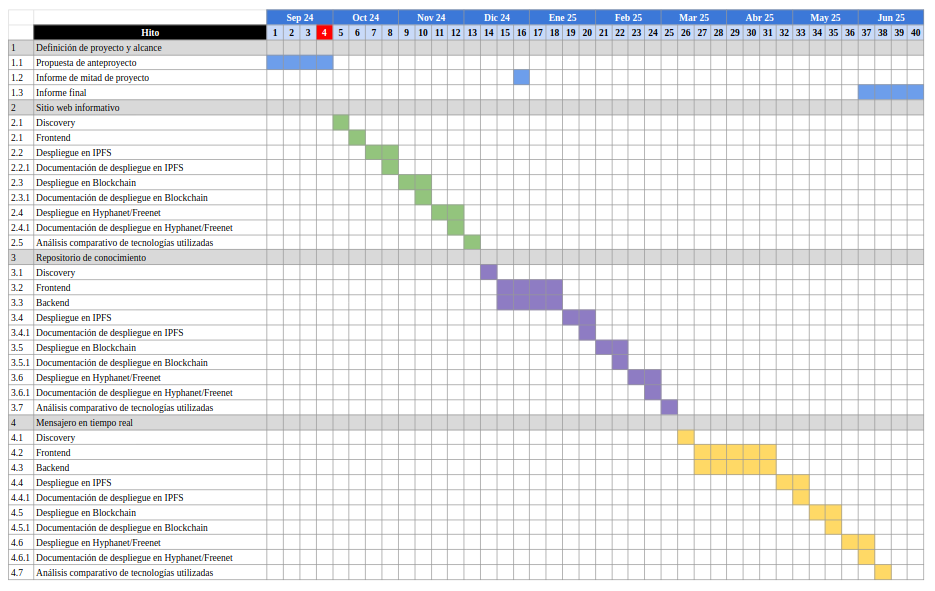
\includegraphics[width=1\linewidth]{img/cronograma.png}
    \caption{Cronograma tentativo}
    \label{fig:cronograma-tentativo}
\end{figure}

Por lo tanto, lo que terminó sucediendo es lo que se muestra en la Figura \ref{fig:cronograma-real}. La división se hizo por ecosistema, esto incluye la investigación, el desarrollo y la documentación de cada caso de uso para el ecosistema en cuestión. Hacerlo de esta manera nos permitió paralelizar los esfuerzos y evitamos superposiciones durante la investigación y desarrollo. Esta separación podría haber generado silos de conocimiento por ecosistema dentro del equipo, es por esto que las reuniones semanales de puesta en común, junto con la constante comunicación por chat y sesiones de \textit{pair-programming}, fueron de vital importancia para mitigar dicha separación y que todo el equipo esté al tanto de los conocimientos adquiridos de cada ecosistema.

\begin{figure}[H]
    \centering
    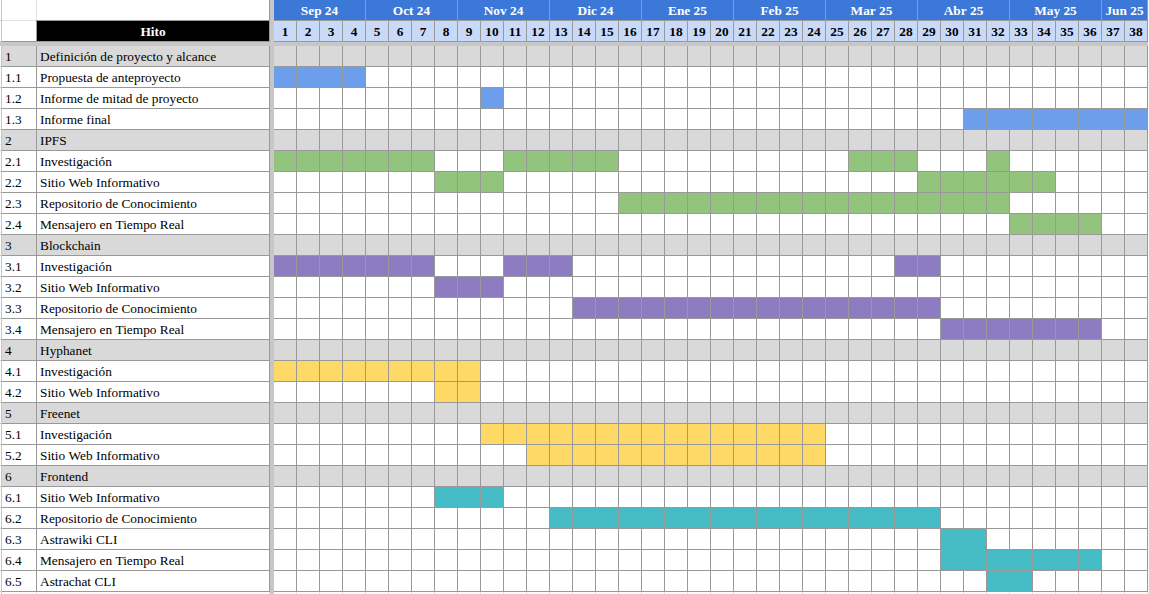
\includegraphics[width=1\linewidth]{img/cronograma-real.png}
    \caption{Cronograma real}
    \label{fig:cronograma-real}
\end{figure}


% \begin{enumerate}

%     \item \textbf{Definición de proyecto y alcance}
%     \begin{enumerate}[label*=\arabic*.]
%         \item Propuesta de anteproyecto (Semanas 1 a 4)
%         \item Informe de mitad de proyecto (Semanas 16 a 17)
%         \item Informe final (Semanas 37 a 40)
%     \end{enumerate}
    
%     \item \textbf{Sitio web informativo} (Semanas 5 a 13)
%     \begin{enumerate}[label*=\arabic*.]
%         \item Discovery
%         \item Frontend
%         \item Despliegue en IPFS
%         \begin{enumerate}[label*=\arabic*.]
%             \item Documentación de despliegue en IPFS
%         \end{enumerate}
%         \item Despliegue en Blockchain
%         \begin{enumerate}[label*=\arabic*.]
%             \item Documentación de despliegue en Blockchain
%         \end{enumerate}
%         \item Despliegue en Hyphanet/Freenet
%         \begin{enumerate}[label*=\arabic*.]
%             \item Documentación de despliegue en Hyphanet/Freenet
%         \end{enumerate}
%         \item Análisis comparativo de tecnologías utilizadas
%     \end{enumerate}
    
%     \item \textbf{Repositorio de conocimiento} (Semanas 14 a 25)
%     \begin{enumerate}[label*=\arabic*.]
%         \item Discovery
%         \item Frontend
%         \item Backend
%         \item Despliegue en IPFS
%         \begin{enumerate}[label*=\arabic*.]
%             \item Documentación de despliegue en IPFS
%         \end{enumerate}
%         \item Despliegue en Blockchain
%         \begin{enumerate}[label*=\arabic*.]
%             \item Documentación de despliegue en Blockchain
%         \end{enumerate}
%         \item Despliegue en Hyphanet/Freenet
%         \begin{enumerate}[label*=\arabic*.]
%             \item Documentación de despliegue en Hyphanet/Freenet
%         \end{enumerate}
%         \item Análisis comparativo de tecnologías utilizadas
%     \end{enumerate}
    
%     \item \textbf{Mensajero en tiempo real} (Semanas 26 a 38)
%     \begin{enumerate}[label*=\arabic*.]
%         \item Discovery
%         \item Frontend
%         \item Backend
%         \item Despliegue en IPFS
%         \begin{enumerate}[label*=\arabic*.]
%             \item Documentación de despliegue en IPFS
%         \end{enumerate}
%         \item Despliegue en Blockchain
%         \begin{enumerate}[label*=\arabic*.]
%             \item Documentación de despliegue en Blockchain
%         \end{enumerate}
%         \item Despliegue en Hyphanet/Freenet
%         \begin{enumerate}[label*=\arabic*.]
%             \item Documentación de despliegue en Hyphanet/Freenet
%         \end{enumerate}
%         \item Análisis comparativo de tecnologías utilizadas
%     \end{enumerate}

% \end{enumerate}
\section{Riesgos materializados}

% Poner la tabla, hay una en el notion 

% \setlength\tabcolsep{3pt}
% \begin{center}
%     % \begin{tabularx}{\linewidth}{*{8}{|c}{>\RaggedRight\arraybackslash}X}
%     % \begin{tabularx}{\textwidth}{|l|c|*{8}{>{\RaggedRight\arraybackslash}X}}
%     \begin{tabular}{*{5}{|p{80pt}}|}
%     \hline
%     \textbf{Descripción} & \textbf{Causa}  & \textbf{Plan \break de Respuesta} & Umbral & Plan de Contingencia \\
%     \hline\hline
%     Incapacidad de utilizar Hyphanet como ecosistema & Documentación desactualizada y/o API poco documentada & Tomar como referencia otras aplicaciones & Las aplicaciones de referencia no siguen un estándar & Descartar Hyphanet y reemplazar por Freenet \\
%     \hline
%     % \end{tabularx}
%     \end{tabular}
% \end{center}

\renewcommand\theadfont{\bfseries}

\begin{table}[!htbp]
    \centering
    \begin{tabular}{*{5}{|p{70pt}}|}
         \hline
         \thead{Descripción} & \thead{Causa} & \thead{Plan \break de Respuesta} & \thead{Umbral} & \thead{Plan \break de Contingencia} \\
         \hline
         Incapacidad de utilizar Hyphanet como ecosistema & Documentación desactualizada y/o API poco documentada & Tomar como referencia otras aplicaciones & Las aplicaciones de referencia no siguen un estándar & Descartar Hyphanet y reemplazar por Freenet \\
         \hline
    \end{tabular}
    \caption{Caption}
    \label{tab:my_label}
\end{table}

\paragraph{Cambio de Hyphanet a Freenet}
A mitad del proyecto resolvimos cambiar el tercer ecosistema elegido (Hyphanet) por su versión más moderna (Freenet). Esto fue debido a que encontramos que la documentación era escasa, los programas realizados para el ecosistema eran unos pocos y cada uno tenía una forma distinta de implementar ciertas cosas. La API tampoco provee facilidades a la hora de gestionar archivos, manejo de comunicaciones, entre otras cosas que consideramos necesarias para los casos de uso.

\paragraph{Freenet en desarrollo}
Un riesgo que teníamos en cuenta eran las modificaciones que podría sufrir Freenet al estar aún en desarrollo. Esto fue de la mano con que la documentación publicada no está actualizada a la última versión.

\paragraph{Baja de Freenet como ecosistema}
Dada la promesa del equipo de Freenet de lanzar una versión estable en el corto plazo -pero que ya llevaba más de un año en ese estado- decidimos poner como límite el mes de febrero de 2025. Llegada la fecha, no hubo ningún anuncio de la versión estable por lo que decidimos descartar el ecosistema y, en cambio, agregar métricas de performance a los otros ecosistemas.
\section{Lecciones aprendidas}

\begin{itemize}
    \item Trabajar con tecnologías emergentes resulta un desafío al encontrarse en desarrollo constante y frecuente. Esto quiere decir que la documentación es escasa, nula o se encuentra desactualizada.
    
    \item Al trabajar con distintos ecosistemas, modularizar en distintos paquetes/librerías cada uno facilita la integración, las pruebas y el cálculo de métricas.

    \item Nos abrió al mundo P2P y web descentralizada, que es una manera distinta de pensar y desarrollar aplicaciones. [TODO LS: desarrollar]

\end{itemize}
\section{Impactos sociales y ambientales}

A continuación se realizará un análisis del posible impacto que pueda tener el uso de estas herramientas, manteniendo la distinción entre ecosistemas.

\subsection{Aplicaciones en IPFS}

\subsubsection{Moderación y Censura}

%TODO: Cambiar falta de roles a optar por decentralización
Nuestras aplicaciones desarrolladas con IPFS carecen de moderación para los artículos y chats. Esto es debido a la falta de roles, necesarios para una moderación efectiva dentro de cada comunidad. Como se vio previamente, las bases de datos que representan artículos o chats son \textit{append-only}, y por lo tanto no hay una manera de eliminar un contenido en particular sin eliminar la base de datos.

Tampoco es sencillo eliminar la base de datos. Tanto en Astrawiki como en Astrachat, cada chat/artículo es único, y por lo tanto no se puede simplemente sobrescribir el contenido con otra base de datos. Por otro lado, la base de datos siempre estará disponible mientras otras personas la alojen.

La manera más factible de eliminar un artículo o chat por completo es a nivel de front-end, o sea, manualmente eliminando resultados de las búsquedas, y no permitiendo la carga de esos artículos o chats específicos. Esto se puede realizar siempre y cuando se tenga acceso al código fuente del front-end utilizado, y se tenga permisos para modificarlo de manera que los usuarios obtengan la nueva versión al usarlo.

Todas las ventajas y limitaciones de IPFS abarcan nuestras implementaciones. En el caso en que un individuo o entidad -como un gobierno, o un ISP- quiera censurar estos recursos, no basta con prohibir un dominio en particular, ya que IPFS es abierto y los CIDs y nombres de IPNS seguirán disponibles. Existen maneras de censurar por CID que explotan componentes de IPFS como la Distributed Hash Table, pero pueden ser mitigados. \cite{censorship-ipfs} Tampoco es útil inhabilitar un gateway en específico, ya que los usuarios pueden optar por usar otra gateway, o directamente acceder mediante su propio nodo de IPFS.

Por otro lado, los nodos de IPFS no son anónimos. El \texttt{PeerID} de cada nodo es permanente y se mantiene cada vez que se inicia. A la vez, se puede relacionar el \texttt{PeerID} de un nodo con una \textit{multiaddress}, y por lo tanto, la IP pública del nodo \cite{privacy-ipfs}. No obstante, incluso obteniendo la IP de uno de los nodos que aloja el contenido, este suele estar disponible en múltiples nodos. Esto incluye a cualquier usuario que utilice la aplicación y gateways que la recuperen, ya que por la naturaleza de IPFS, el contenido se mantendrá en la caché del nodo por un tiempo.

La contra-cara de estas dificultades para censurar un contenido alojado en IPFS es la facilidad para confirmar que un contenido ya no está disponible. Un nodo puede saber con certeza que un contenido no está disponible simplemente intentando recuperarlo, lo cuál es difícil de lograr con servidores HTTP \cite{doan2022decentralisedcloudstorageipfs}.

Además, un estudio realizado en Septiembre de 2023 \cite{Balduf_2023} afirma que gran parte de los nodos presentes en la red de IPFS provienen de servicios de cloud, los cuáles son propietarios y fáciles de manipular para censurar o restringir el acceso a un contenido en específico. Entre otras estadísticas, se resalta que un 79,6\% de los nodos en la DHT provienen de datacenters, y un 80\% de los nodos que están detrás de una red con NAT, obtienen contenido mediante relays alojados en servicios de cloud. 

Los servicios desarrollados con IPFS como infraestructura son muy resilientes a posibles ataques. A su vez, la dificultad para eliminar contenido no deseado presenta un posible problema, ya que se puede utilizar para alojar contenido malicioso, ilegal, o simplemente no acorde a una comunidad que aloje una wiki o chat.

\paragraph{Acceso a información en regiones con censura o poca conexión} Un beneficio claro del uso de IPFS es su tolerancia a la partición de la red \cite{doan2022decentralisedcloudstorageipfs}. Debido a que el contenido puede ser replicado en múltiples nodos, no se puede completamente limitar el acceso y publicación de contenido. Por otro lado, una vez que un nodo en una red local o regional obtiene el contenido, este estará disponible en esa red mientras el nodo lo ofrezca, lo cuál es útil para lugares en donde la conexión a Internet es limitada, ya que para obtener dicho contenido no se requiere recuperar archivos fuera de la red local.

\subsubsection{Impacto ambiental}

No hay análisis realizados acerca de la utilización de energía por parte de la red de IPFS en comparación con soluciones centralizadas. Sin embargo, hay varios factores que diferencian el uso de energía de una solución centralizada con una realizada con IPFS como infraestructura.

\paragraph{Recuperación de contenido} En un escenario óptimo, el contenido requerido está disponible en un nodo cercano. Por ejemplo, si otro usuario en un área especifico accede a un contenido, el resto de los nodos en ese área podrán recuperar el contenido desde ese nodo. En cambio, un contenido alojado en un servidor HTTP siempre requiere acceso al servidor, el cuál puede estar a mayor distancia. Esto implica un uso mayor de ISPs regionales y de \textit{tier 1}, y en general requiere infraestructura de red de mayor capacidad.

\paragraph{Eficiencia} Dado que parte de los nodos proveedores de contenido están ubicados en la \textit{periferia} de la red (dispositivos móviles, computadoras de hogar, etc.), los métodos de lectura y escritura de contenido no es óptimo. Los nodos pueden estar utilizando discos duros en vez de unidades de estado sólido, o en general componentes ineficientes comparados con un servidor dedicado a proveer contenido HTTP. Esto puede resultar en un mayor uso de energía.

\paragraph{Escalabilidad} Si bien los servicios de cloud proveen escalabilidad para variar la cantidad de máquinas dedicadas a proveer un contenido especifico, la naturaleza de IPFS hace que esta red sea incluso más optimizada. Cuando muchos nodos requieren de un contenido, se replica por la red fácilmente y sin cargas altas para ningún nodo en particular.

Realizar un análisis detallado del impacto ambiental de IPFS es uno de los trabajos futuros propuestos.

\subsection{Aplicaciones en Ethereum}

Se sabe que blockchain abrió un mundo de posibilidades en cuanto a la privacidad y el impacto ambiental. A continuación desarrollaremos el impacto de las aplicaciones desarrolladas en esta tecnología.

\subsubsection{Moderación y Censura}

Al igual que como sucede con IPFS, en Ethereum no es posible borrar un \textit{smart contract} de la red. Esto significa que una vez creado un artículo o un chat el mismo no puede ser borrado, haciéndolo resistente a la censura.

En cuanto a la moderación de contenido por parte de gobiernos o ISP, no es posible dado que es una red distribuida y, mientras exista un nodo que tenga la información de la red, la misma va a estar disponible para todos los usuarios.

Si se trata de moderación de contenido por parte de los propios usuarios no se puede garantizar que no surjan modificaciones en los artículos o chats. Cualquier persona con la \textit{address} del contrato y cumpliendo con la firma de los métodos del mismo puede realizar modificaciones.

\subsubsection{Impacto ambiental}

Desde su adopción, blockchain en general ha sido criticado por el enorme impacto ambiental y la huella de carbono al utilizar casi tanta energía eléctrica como un país entero \cite{ethereum-honduras}. Esto, con los años ha ido cambiando y, al día de hoy, existen blockchains \textit{eco-friendly}\cite{blockchain-eco-friendly}. En particular, la red de Ethereum pasó de utilizar \textit{proof-of-work} a \textit{proof-of-stake} lo cual hizo que el consumo eléctrico de los nodos disminuyera en hasta un 99\%\cite{ethereum-green}. Sin embargo, hay dudas sobre la forma de medir este impacto y compararlo con otras blockchain como Bitcoin. Además, la cantidad de nodos que se sumaron a \textit{proof-of-stake} luego de la migración se duplicó.\cite{ethereum-pos}

\section{Trabajos futuros}

En base al análisis realizado, se detectaron diversas lineas de trabajo futuras de las cuales se puede continuar el desarrollo.

\subsection{Mejoras a los casos de uso}

A continuación se proponen mejoras para los casos de uso implementados, los cuales, por temas de tiempo, no se llegaron a implementar.

\subsubsection{Astrawiki-eth}

Teniendo en cuenta que es el caso de uso donde mayor volumen de datos se transfieren, por lo tanto mayor costo de gas, una mejora involucra la disminución de este costo. Se podría disminuir haciendo uso de los clones de \textit{smart contract}s según lo propuesto en el ERC-1167\cite{erc-1167}. En resumen, lo que se propone es que haya un contrato como ''plantilla'' al cual se lo copia cada vez que, por ejemplo, se crea un artículo nuevo.

\subsubsection{Astrachat-eth}

Una de las principales mejoras que se pueden implementar sobre este caso de uso es respecto a la experiencia de uso para frontends en navegadores web. El hecho que para cada mensaje enviado sea necesario confirmar una transacción por medio de la wallet hace que la aplicación pierda el factor de \textit{real-time}. Una posible solución a este problema es que se pueda crear un balance en un fondo común (con dinero de los usuarios) de forma que cada vez que se envíe un mensaje se tome de este fondo para pagar la transacción. Esta mejora haría más fácil la integración con otros frontends que no corren en navegadores web como \textit{Astrachat-cli} aunque también queda investigar cómo conectar una wallet a los mismos.

Por otro lado, en base al costo por transacción (visto en la sección \ref{performance-blockchain}) se podría utilizar alguna red cuyos precios de gas por transacción sean menores. Una de estas redes --basada en Ethereum-- es la \textit{Ronin Network}\cite{ronin-network}\cite{ronin-network-whitepaper} que a principio de este año (2025) abrió su red para que cualquier usuario pueda implementar aplicaciones en la misma.

\subsection{Mejora para clusters colaborativos}

Como se mencionó previamente en el análisis de IPFS, los clusters colaborativos son una alternativa para lograr la persistencia y disponibilidad de archivos, a través del "pinneo" de nodos colaborativos. La cual va muy de la mano con la filosofía de las aplicaciones comunitarias, ya que potencialmente la propia gente que utiliza la aplicación sea la que la mantenga colaborativamente. El problema es que actualmente casi no se utiliza esta alternativa, lo cual lleva a que por ejemplo, no haya una manera fácil de utilizarla, sin embargo esto tiene sus razones.

\paragraph{IPFS Cluster}

Para entender mejor por qué no se utiliza mucho esta forma de "pineo" y cuales son sus limitaciones, primero hay que entender que es lo que se utiliza. IPFS cuenta con una aplicación distribuida llamada IPFS Cluster, esta funciona a la par de los nodos de IPFS y permite mantener un conjunto global de "pines", alocando inteligentemente los items a sus nodos.

Gracias a esta aplicación es posible la creación de clusters colaborativos. Los clusters colaborativos permiten que \textit{peers} individuales, que no son de confianza, se unan a un clúster IPFS como "seguidores" (sin permiso para modificar o editar el conjunto de pines).

Para crear este cluster es necesario primero contar con algunos nodos confiables, aquellos que van a tener permitido modificar qué archivos son los que pertenecen al conjunto de "pines". Y es esta nuestra primera limitación, ya que no se puede permitir que cualquier nodo pueda modificar este conjunto, entonces es necesario contar con nodos propios que tengan ese rol.

Otra cosa muy importante que se puede configurar sobre el cluster es el \textit{replication factor}, este ajuste permite indicar a cuantos nodos se va a replicar cada archivo. Esto es muy importante porque permite que no sea obligatorio replicar la totalidad de los archivos en todos los nodos. 

Sin embargo existe una limitación muy importante, IPFS Cluster no verifica si los seguidores realmente están "pineando" o no el contenido, ni cuánto espacio tienen ni otras métricas. Confía en todo lo que dicen. Eso significa que un seguidor malintencionado siempre puede fingir que tiene suficiente espacio, que se le asignen pines o fragmentos, pero al final no "pinea" nada. Un grupo formado por voluntarios aleatorios y que no son de confianza no puede usar, por ejemplo, factor de replicación de tres, porque esos 3 miembros podrían simplemente estar fingiendo "pinear" cosas. Es por eso que el escenario que mejor funciona es dejando que todos "pineen" todo y esperar que algunos de los \textit{peers} no sean maliciosos.

Justamente de esa manera es como funcionan los clusters públicos actualmente, visibles en la página de IPFS\cite{collaborative-clusters}, donde hay algunos que piden gigabytes, y hasta algunos terabytes de información, para poder colaborar. Esto es algo totalmente inviable para que la gente pueda colaborar hasta un cierto almacenamiento, limitando mucho la posibilidad de distribución de colaboradores.

\paragraph{Deployado, seguimiento y descubrimiento}

Habiendo hablado ya de las limitaciones más técnicas que se prensentan al usar cluster colaborativos, hay otro tipo de limitación que es el la falta de facilidad a la hora de deployar, seguir y descubrir aplicaciones colaborativas que usen IPFS cluster.

En primer lugar hablemos del deployado, actualmente si se quiere deployar la aplicación en un cluster colaborativo la única forma que existe es hacerlo de forma manual y crear un servicio que se ocupe de actualizar el conjunto de "pines" cuando sea necesario actualizarse. Si bien es factible, no es algo cómodo para todos y limita a decidirse ir por este camino. Lo ideal sería, que exista un servicio, parecido al ofrecido en los servicios de \textit{pinning}, como es el caso de Fleek\cite{fleek}, donde al actualizar el repositorio ya se deployen los cambios. Facilitando asi su deployado en el cluster colaborativo. Se podría pensar como un servicio que corra sobre los nodos \textit{trusted} donde, cuando un nodo lider detecte que se hizo un cambio, se "buildee" la página web por ejemplo, y se despliegue en el cluster comunitario.

Parecido a lo anterior, alguien que quiera colaborar necesita ejecutar comandos manualmente que para mucha gente no sabe lo que está haciendo, lo cual también termina desincentivando y generando que menos gente decida por colaborar.

Por último no existe una manera fácil de presentar y descubrir nuevos o existentes proyectos comunitarios que la gente pueda optar por colaborar. Actualmente el único lugar donde prensentan proyectos públicos para colaborar es la página de IPFS\cite{collaborative-clusters}, que ademas se ser bastante simple, depende de ellos si agregan un nuevo proyecto para presentar en esa página. Donde lo ideal sería que puedan publicarse nuevos proyectos junto a una descripción y que la gente pueda conocerlos y optar por colaborar de una manera mucho más sencilla.

\paragraph{Conclusión}

Con esto concluimos que se presenta la oportunidad para una linea de trabajo futura focalizada en la mejora para clusters colaborativos. 

En primer lugar una mejora técnica donde se modifique o se construya por encima de IPFS cluster, que permita principalmente que en un clúster comunitario se asegure el "pineo" de información sin necesidad de tener que obligar a todos los colaboradores a "pinear" la totalidad de los archivos.

En segundo lugar, la creación de una plataforma o aplicación, que permita la facilitación del deployado, seguimiento y descubrimiento de aplicaciones colaborativas.

\subsection{Análisis del consumo de energía en la red de IPFS}

Como se mencionó anteriormente, no hay análisis detallado del uso de energía en la red de IPFS. Un posible trabajo involucra calcular una huella de carbono aproximada, el consumo promedio de energía, entre otras métricas. De ello puede desprenderse un análisis comparativo entre diferentes ecosistemas como Blockchain, y cloud hosting tradicional.

\subsection{Blockchain para aplicaciones comunitarias}

En la búsqueda de una blockchain comunitaria nos encontramos con un servicio llamado \textit{Filecoin}\cite{filecoin} el cual provee de incentivos monetarios para aquellos que cedan espacio en sus discos a guardar archivos de otras personas. Es abierto para que cualquier persona pueda unirse a la red peer-to-peer que proveen. Funciona por arriba de IPFS, utiliza tecnologías de Blockchain para los incentivos y dar garantía que los datos están realmente guardados en los nodos. Nuestra propuesta de trabajo futuro es que se cree una tecnología basada en Blockchain que no necesite del incentivo monetario para funcionar y que además permita la ejecución de código.

\subsection{Análisis de Freenet como ecosistema}

Si en un futuro Freenet finalmente sale en una versión estable, creemos que sería un buen ecosistema al cual realizar un análisis como el de este trabajo y hasta más en profundidad con otro tipo de aplicaciones distribuidas y descentralizadas.

\section{Conclusiones}

Luego de todo el análisis realizado podemos ver que cada ecosistema tiene sus ventajas y desventajas. IPFS y Swarm por su naturaleza como almacenamientos descentralizados funcionan muy bien para sitios web estáticos. En particular, IPFS tiene la gran ventaja de no requerir costos monetarios para el usuario final, si no que promueve la colaboración a través de la donación de almacenamiento. Por otro lado, Ethereum y Swarm sí requieren un costo monetario para el usuario final pero aseguran una disponibilidad y persistencia mucho mayor. Ethereum resulta útil para aplicaciones como el repositorio de conocimiento y el mensajero en tiempo real pero se puede volver muy costoso según su implementación, además de algunas cuestiones de usabilidad que son más evidentes en el mensajero. Además, debido a su comunidad y amplia documentación, Ethereum presenta una mejor experiencia de usuario que el resto de ecosistemas. Por su parte, Hyphanet se encuentra prácticamente abandonado y su proyecto sucesor Freenet, si bien parece prometer, todavía está en pleno desarrollo. Concluyendo en que lo más beneficioso sea combinar lo mejor de cada ecosistema para aplicaciones como los casos de uso presentados.

El desarrollo de este trabajo nos brindó la oportunidad de explorar estas tecnologías emergentes las cuales, al estar en desarrollo constante, presentaron varios desafíos que tuvimos que afrontar como la ausencia de documentación o documentación desactualizada, cambios repentinos de la interfaz de ciertas librerías, faltas de herramientas necesarias para el desarrollo o despliegue de algún ecosistema (lo visto en IPFS), o incluso tecnologías que todavía se encuentran en desarrollo y no tienen una versión estable (como nos sucedió con Freenet). Por otra parte, logramos aplicar los conocimientos técnicos adquiridos en nuestra formación académica y nos adentramos en la comunidad \textit{open source}.

Por último, hoy podemos decir que adquirimos nuevas herramientas y conocimientos que previamente no poseíamos en la profundidad alcanzada en este trabajo y que, sin duda, podremos aplicar en el futuro.

\section{Referencias}
\printbibliography[heading=none]
\section{Anexos}
\subsection{Herramientas de LibP2P utilizadas}
\subsection{Arquitectura del repositorio de conocimiento}

La arquitectura del repositorio de conocimiento fue diseñada de manera independiente del ecosistema utilizado. Se tomó esta decisión para proveer una interfaz común, independiente de su implementación en IPFS y Ethereum. De esta manera, una aplicación puede trabajar sobre una API común e intercambiar implementaciones fácilmente. Esto es útil para la implementación del front-end del repositorio, como se verá más adelante.

En sí, la arquitectura consiste de una o varias \textit{wikis}, dependiendo de la implementación. Cada wiki se identifica con un nombre único que representa un grupo de artículos en conjunto. Cada wiki se representa con una lista de artículos, los cuales son identificados por sus nombres —también únicos. 

Un artículo se compone de un nombre único y no vacío y su contenido. Si bien nuestra implementación utiliza \textit{markdown} \cite{markdown} como formato del contenido, el tipo de contenido es arbitrario e indiferente para la wiki, cualquier tipo de archivo es admisible. Únicamente será tenido en cuenta en el momento en el que la aplicación que interactúe con el contenido lo interprete. En nuestro caso, markdown representa una manera sencilla de enriquecer un texto, lo cual lo hace apropiado para un repositorio de conocimiento comunitario.

\begin{figure}[H]
    \centering
    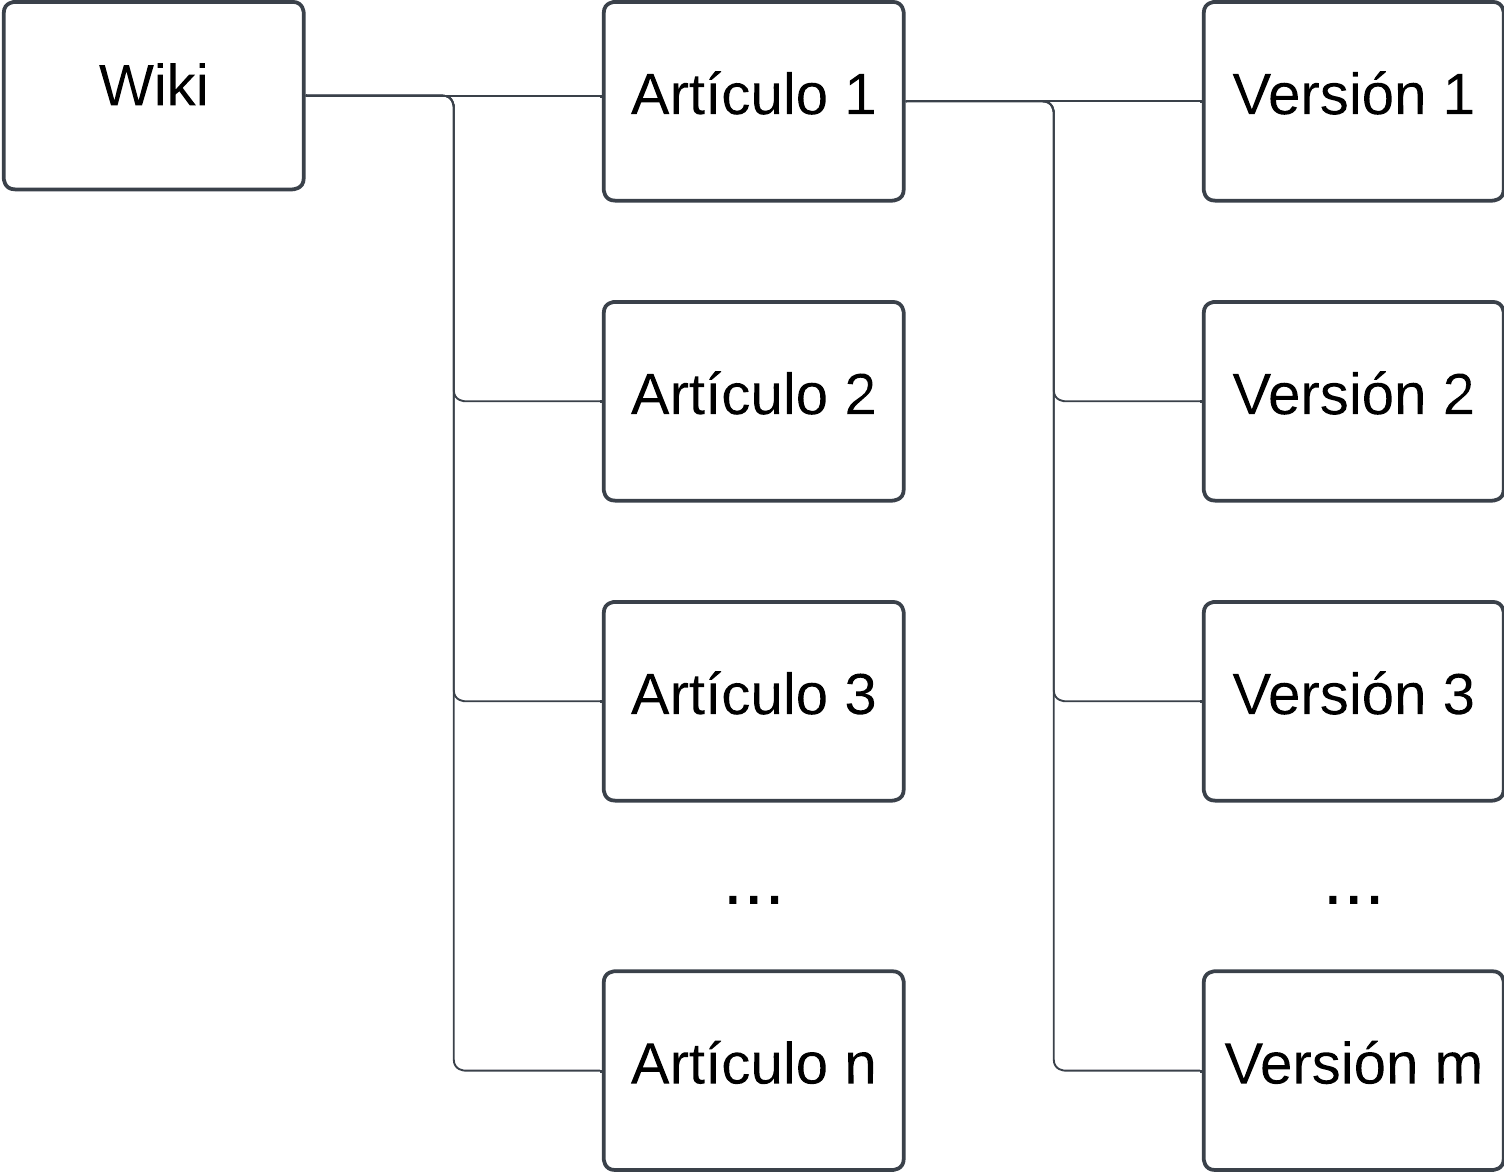
\includegraphics[width=0.5\linewidth]{img/solucion-wiki/arquitectura-wiki.png}
    \caption{Arquitectura general del repositorio de conocimiento.}
    \label{fig:architecture-wiki}
\end{figure}

\subsubsection{Representación de un artículo}

Internamente, los artículos pueden editarse en el tiempo, y un usuario debe obtener siempre la última versión. Sin embargo, se debe poder ver versiones anteriores si así lo desea el usuario, por lo que guardar la última versión únicamente no es válido. Es por esto que se decidió representar a un artículo como un nombre, y un conjunto de versiones. Cada versión representa una modificación hecha al artículo. Un artículo nuevo tendrá una única versión, y al hacerle una edición tendrá dos.

Esta iteración de la arquitectura permite a los usuarios ver el historial de versiones, y acceder a cualquiera de ellas. Pero guardar todo un artículo por cada edición puede ser costoso en concepto de almacenamiento. Rara vez un artículo es modificado en su totalidad \cite{wiki-edits-stats}. En cambio, las ediciones que puede sufrir un artículo se deben en su mayoría a la inclusión de contenido nuevo, o la modificación de una sección en particular. Guardar el contenido completo en casos donde los cambios son mínimos resulta ineficiente, y es particularmente negativo en aplicaciones peer-to-peer, donde el contenido se almacena en el lado del usuario.

\paragraph{Generación de patches}

Como solución para minimizar la información redundante en cada versión, se decidió usar el tipo de algoritmo de \textit{data differencing} \cite{data-differencing}, que consiste en almacenar únicamente los cambios hechos en una versión con respecto a su antecesora, de forma similar a \textit{Git}. Esta lista de cambios forma un \textit{patch}.

Un patch se obtiene al aplicar un algoritmo que reciba el contenido anterior, y el contenido nuevo, y devuelva un patch que pueda ser utilizado posteriormente para reconstruir el contenido. Si bien hay varios algoritmos que logran este objetivo, se decidió utilizar el algoritmo de diff de Myers \cite{myers-diff}, ya que ofrece un punto medio entre compresión, y cómputo necesario para compilar el texto. Este algoritmo es el que utiliza la biblioteca diff-match-patch, creada por Google, que ofrece una interfaz sencilla para lograr generar patches y luego compilar texto en base a ellos.

Calculando los patches de la nueva versión con respecto a la anterior, reducimos el espacio necesario para almacenar un artículo con todas sus versiones.  Hay casos en los que un patch puede tener un tamaño mayor al de simplemente almacenar una copia del nuevo contenido. Sin embargo, estos casos no son frecuentes en usos comunes y decidimos despreciarlos, aunque puede ser una posible mejora para optimizar más aún el espacio utilizado.

Por otra parte, ya que cada versión no tiene toda la información, se necesitan todas las versiones anteriores para compilar el contenido resultante. Esto puede ser una desventaja en archivos con muchas ediciones, ya que requieren de mayor cómputo para compilar, específicamente \texttt{O(n)}, donde \texttt{n} es la cantidad de versiones que tiene el artículo. Para mejorar esto, una posible mejora consiste en fijar un número máximo de patches consecutivos que, al superarse, indica que la siguiente versión debe contener el contenido completo. De esta manera se acota la cantidad de iteraciones que puede tomar la compilación de un artículo.

La nueva iteración de la arquitectura apunta a tener una lista de versiones, que a su vez contengan el patch con las diferencias con la versión anterior. Pero como se verá en la siguiente sección, esta solución no es lo suficientemente resiliente.

\subsubsection{Concurrencia}

En las redes peer-to-peer es común que la replicación de contenido lleve un tiempo no despreciable. Esto puede generar problemas, ya que dos nodos pueden publicar contenido que entre en conflicto, de la misma manera que dos cambios pueden generar un \textit{merge conflict} en Git. En el mejor de los casos, ambos nodos publican
contenido que no entra en conflicto entre sí, y por lo tanto la compilación se puede realizar sin problemas. En el caso contrario, puede dejar el artículo en un estado inválido, imposible de compilar y por lo tanto, inaccesible.

Yendo a nuestro caso de uso, el problema planteado previamente puede entrar en conflicto de dos maneras:
\begin{enumerate}
    \item Al crear un articulo
    \item Al editar un artículo
\end{enumerate}

Por lo tanto, es necesario una solución que mitigue estos problemas.

Para el caso de la creación de dos artículos con en mismo nombre, se delega en cada ecosistema la responsabilidad de detectar estos casos y actuar en consecuencia. La implementación de cada ecosistema contiene más información para tomar una decisión optimizada al respecto, la cuál se verá en secciones posteriores. En cambio, el problema de la edición de un artículo de forma concurrente puede ser resuelto a nivel arquitectura.

\subsubsection{Árbol de versiones}

Hasta ahora, cada versión se agrega a una lista de versiones, y se asume que cada versión se basa en la anterior. Cuando ocurre un conflicto de concurrencia entre versiones, esto no aplica por las razones dadas previamente. Por lo tanto, es necesario que cada versión tenga un ID para que las versiones posteriores puedan mantener registro de su versión padre, es decir, la versión sobre la que se basa. Todas las versiones tienen padre, excepto la versión inicial. Cuando dos versiones se crean en base a una misma versión padre, se genera una bifurcación. Por lo tanto, las versiones pasan a formar un árbol.

En arquitecturas tradicionales, la generación de IDs suele hacerse por la misma base de datos, de manera incremental. Esto no genera problemas ya que el servidor decide en que orden tomar las versiones. En una aplicación distribuida, esto no es conveniente, ya que dos nodos pueden generar el mismo ID por la misma razón por la que pueden generar versiones conflictivas. La solución elegida fue usar \texttt{UUID}s \cite{uuid}, que se generan sin necesidad de centralizar la decisión, y tienen una probabilidad de colisión casi nula.

Una problemática que trae tener distintas ramas de versiones es que la compilación del contenido deja de ser trivial, ya que hay múltiples posibles últimas versiones, dependiendo de la rama que se elija. Para resolver esto es necesario definir una heurística que elija la rama principal del artículo de forma determinista.

\begin{figure}[H]
    \centering
    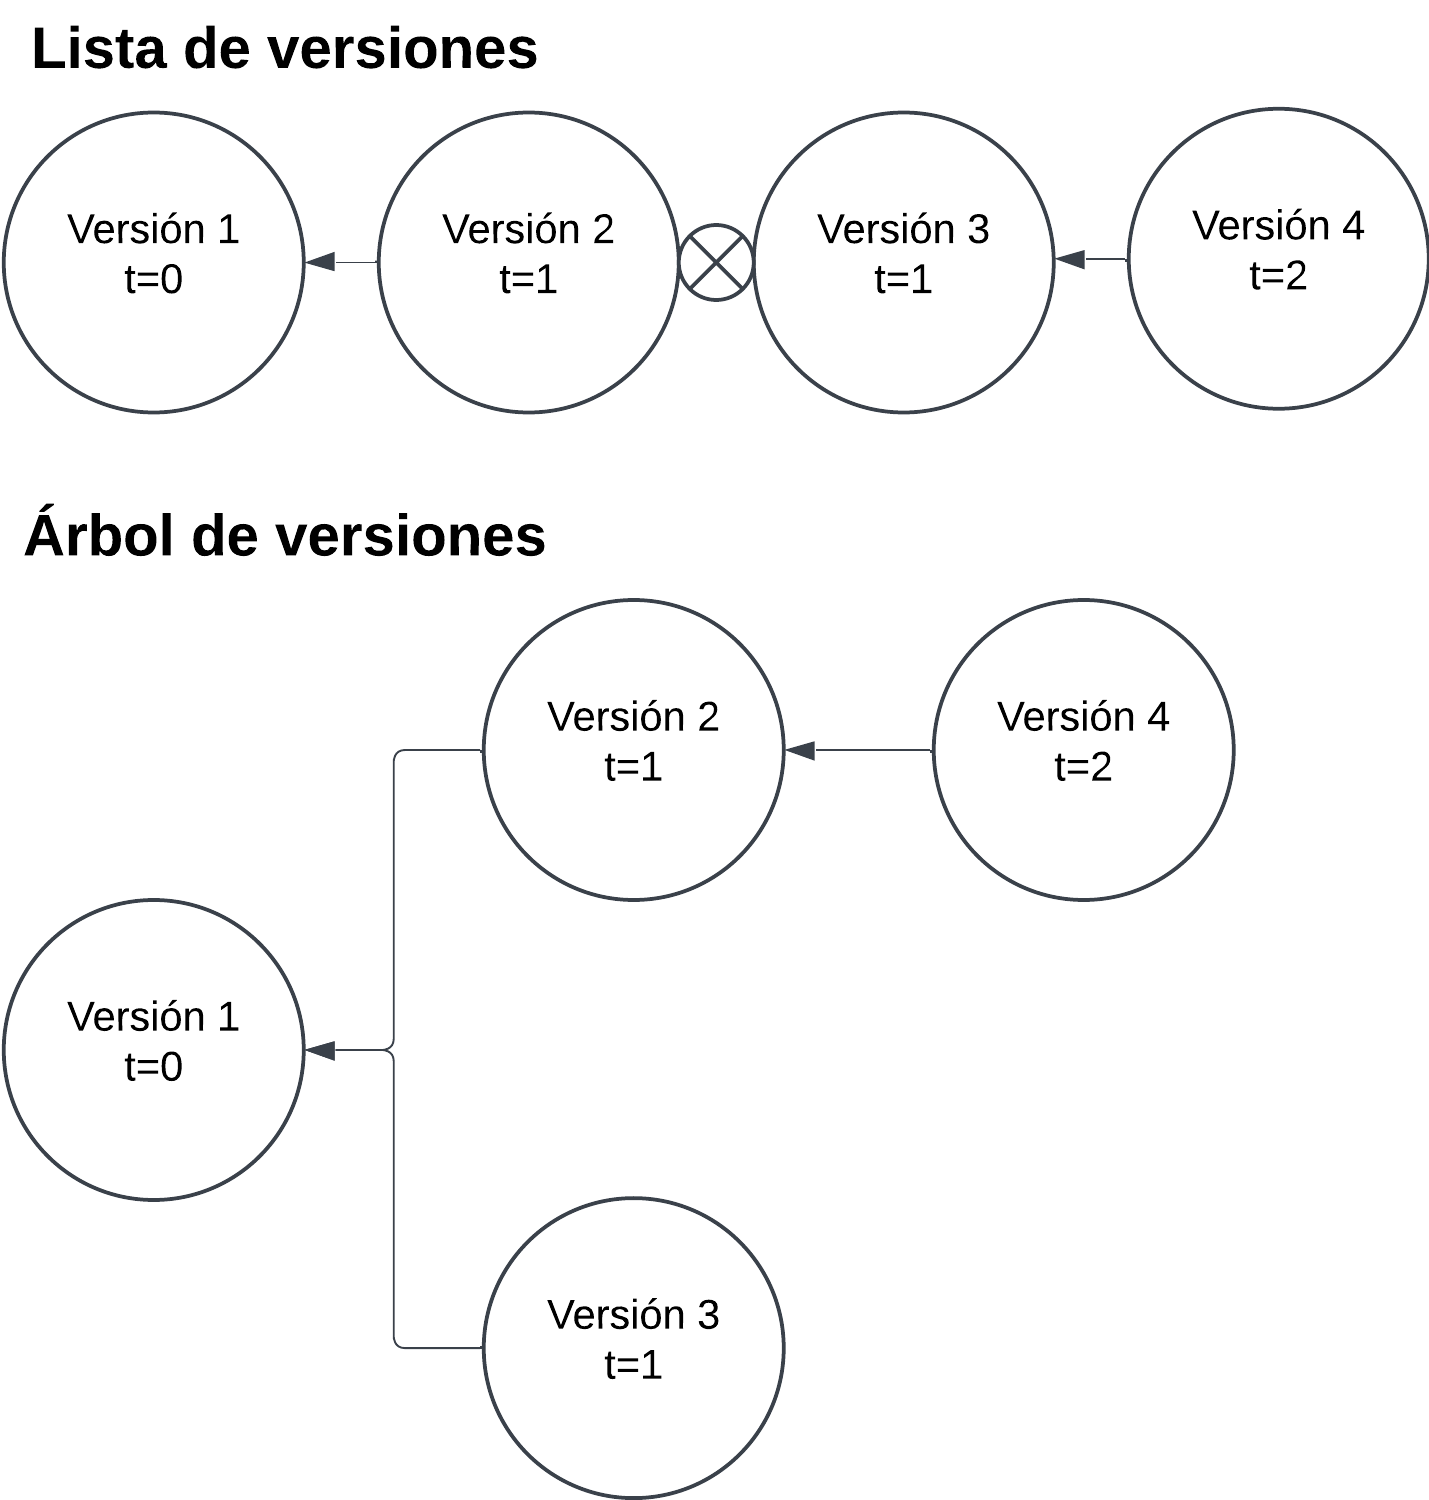
\includegraphics[width=0.5\linewidth]{img/solucion-wiki/arbol-versiones.png}
    \caption{Ambas maneras de almacenar versiones. En este caso, \texttt{t} es un momento en el tiempo en el que todas las bases de datos están sincronizadas. En el primer caso, cuando \texttt{t=1} en ambas versiones, significa que hay un conflicto ya que ambas se basan en la misma versión padre. En el árbol, ese problema se mitiga.}
    \label{fig:versions-tree}
\end{figure}

\paragraph{Elección de rama principal}

Una de las decisiones tomadas respecto al árbol de versiones, es que los usuarios sólo puedan modificar la última versión “principal”, es decir; un usuario no podrá editar en base a una versión arbitraria. Teniendo en cuenta esto, es fácil deducir que las ramas no principales o secundarias tendrán a lo sumo una versión en la mayoría de los casos. Esto es debido a que los demás usuarios que no hayan causado la colisión elegirán una rama principal, por lo tanto las demás ramas dejarán de recibir versiones nuevas. Elegir la rama de mayor cantidad de versiones será parte de la heurística para elegir la rama principal.

Sin embargo, esta decisión no es exhaustiva, ya que puede haber dos ramas con la misma longitud. De hecho, este caso es muy común debido a que dos usuarios que crean una nueva versión en base a la misma versión padre generan dos ramas del mismo tamaño. Para tomar una decisión que sea determinista e igual en todos los nodos, se decidió tomar la antigüedad de la última versión de cada rama como parámetro para la heurística. La rama mas antigua será considerada la rama principal. La antigüedad de una rama es decidida por una marca de tiempo o \textit{timestamp} grabada en el mismo nodo que crea la rama, y es enviado como parte de la versión a los demás nodos. Esto trae una desventaja en cuánto a seguridad, ya que un nodo puede falsificar un timestamp y así tener prioridad siempre, pero es mejorable utilizando algoritmos para crear timestamps en un sistema distribuido \cite{distributed-timestamps}.

\begin{figure}[H]
    \centering
    \begin{minipage}{0.9\linewidth}
        \lstset{
            basicstyle=\ttfamily\small,
            frame=single,
            captionpos=b
        }
        \begin{lstlisting}
type VersionID = string;

type Version = {
  id: VersionID;
  date: string;
  patch: Patch;
  parent: VersionID | null;
};\end{lstlisting}
    \end{minipage}
    \caption{Propiedades de una \texttt{Version}}
    \label{fig:version-type}
\end{figure}

Una vez elegida la versión principal, se considera como rama principal a todas las versiones que entren en la cadena de padres, empezando por la versión principal hasta llegar a la versión raíz. De esta forma, sabemos que la rama principal siempre se podrá compilar, generando una red mucho más resiliente a cambios concurrentes. 
Por último, las versiones que no sean parte de la rama principal también podrán visualizarse. Se tomó esta decisión para permitir que los usuarios que hayan subido una versión por fuera de la rama principal puedan ver el contenido que editaron y, en todo caso, editar la nueva versión principal con el mismo.

\subsubsection{Arquitectura del mensajero en tiempo real}

La arquitectura para un mensajero es mucho más sencilla que la del repositorio de conocimiento. Consta de un grupo de chats, que a su vez contienen todos los mensajes. Cada mensaje contiene el texto enviado, el usuario que lo envió, un \textit{timestamp} del momento de su envío, entre otras cosas.

\paragraph{Aliases} En las implementaciones que se verán posteriormente, se determina que la manera de identificar a un usuario será mediante un ID similar a un hash en ambos casos. Esto es común para sistemas descentralizados, pero vuelve difícil diferenciar los usuarios en un chat. Para solucionar esto, se decidió agregar un alias que identifique al usuario, que no tenga que ser único y pueda ser cambiado. Su implementación varía dependiendo del ecosistema, pero en ambos es parte del objeto \texttt{ChatMessage} que almacena cada chat.

\paragraph{Respuestas} Se decidió identificar cada mensaje mediante un identificador, de manera tal que se pueda indicar el "padre" de un mensaje, o sea, el mensaje al que se le está respondiendo.

\begin{figure}[H]
    \centering
    \begin{minipage}{0.9\linewidth}
        \lstset{
            basicstyle=\ttfamily\small,
            frame=single,
            captionpos=b
        }
        \begin{lstlisting}
export type ChatMessage = {
  id: string;
  parentId: string;
  sender: string;
  senderAlias: string;
  message: string;
  timestamp: number;
};\end{lstlisting}
    \end{minipage}
    \caption{Propiedades de un \texttt{ChatMessage}}
    \label{fig:chat-message}
\end{figure}
\newpage
\end{document}